\documentclass[10pt]{article}
\usepackage[vietnamese]{babel}
\usepackage[utf8]{inputenc}
\usepackage[T5]{fontenc}
\usepackage{amsmath}
\usepackage{amsfonts}
\usepackage{amssymb}
\usepackage[version=4]{mhchem}
\usepackage{stmaryrd}
\usepackage{graphicx}
\usepackage[export]{adjustbox}
\graphicspath{ {./images/} }
\usepackage{caption}
\usepackage{hyperref}
\hypersetup{colorlinks=true, linkcolor=blue, filecolor=magenta, urlcolor=cyan,}
\urlstyle{same}
\usepackage{multirow}

\def\AA{\mathring{\mathrm{A}}}

\begin{document}
\captionsetup{singlelinecheck=false}
\section*{CÂU HỎI VÀ BÀI TẬP}
\section*{BET}
\section*{NHẬP MÔN HOÁ HOC}
1.1. Những nội dung nào dưới đây thuộc đối tượng nghiên cửu của hoá học?\\
A. Sự vận chuyển của máu trong hệ tuần hoàn.\\
B. Sự tự quay của Trái Đất quanh trục riêng.\\
C. Sự chuyển hoá thức ăn trong hệ tiêu hoá.\\
D. Sự phá huỷ tầng ozone bởi freon-12.\\
1.2. Điền từ/ cụm từ thích hợp vào chỗ trống trong những câu sau:\\
a) Hoá học là ngành khoa học thuộc lĩnh vực ...(1)..., nghiên cứu về thành phần, cấu trúc, tính chất, sự biến đổi của các đơn chất, hợp chất và ...(2)... đi kèm những quá trình biến đổi đó.\\
b) Hoá học kết hợp chặt chẽ giữa lí thuyết và ...(1)..., là cầu nối giữa các ngành khoa học tự nhiên khác. Hoá học có ...(2)... nhánh chính. Đối tượng nghiên cứu của hoá học là ...(3)...\\
1.3. Tinh bột là nguồn dưỡng chất quan trọng cho cơ thể con người. Các nguyên tố tạo nên tinh bột là:\\
A. H, C, O.\\
B. $C, O, K$.\\
C. O, C, P.\\
D. C, O, N.\\
1.4. Hãy chỉ ra sự khác nhau về cấu tạo của hai hydrocarbon có cùng công thức phân tử $\mathrm{C}_{5} \mathrm{H}_{12}$ sau đây:

\[
\begin{array}{ll} 
& \mathrm{CH}_{3}-\mathrm{CH}_{2}-\mathrm{CH}_{2}-\mathrm{CH}_{2}-\mathrm{CH}_{3} \\
\text { và } & \left(\mathrm{CH}_{3}\right)_{4} \mathrm{C} \tag{2}
\end{array}
\]

Nhiệt độ sôi của hai chất này là bằng nhau hay khác nhau? Vì sao?\\
1.5. Em hãy chỉ ra một số lí do để giải thích vì sao bên cạnh việc nhận thức kiến thức hoá học từ sách vở và thầy cô thì các hoạt động khám phá thế giới tự nhiên dưới góc độ hoá học cũng như vận dụng kiến thức hoá học vào thực tiễn lại có ý nghĩa quan trọng trong việc học tập môn Hoá học. Nêu ví dụ minh hoạ.\\
1.6. Em hãy trình bày vai trò của hoá học trong thực tiễn. Nêu ra các ví dụ minh hoạ khác trong sách giáo khoa (SGK).

\section*{CHỦ DỀ 1: CẤU TẠO NGUYÊN TỬ}
\section*{Bet 2}
THÀNH PHẦN CỦA NGUYÊN TỬ\\
2.1. Phát biểu nào sau đây là không đúng?\\
A. Tất cả các nguyên tử đều có proton, neutron và electron.\\
B. Proton và electron là các hạt mang điện, neutron là hạt không mang điện.\\
C. Electron tạo nên lớp vỏ nguyên tử.\\
D. Số lượng proton và electron trong nguyên tử là bằng nhau.\\
2.2. Chọn từ thích hợp điền vào chỗ trống trong mỗi phát biểu sau.\\
a) Trong nguyên tử, khối lượng tập trung chủ yếu ở ......\\
b) Kích thước hạt nhân rất ...... so với kích thước nguyên tử.\\
c) Trong nguyên tử, phần không gian ...... chiếm chủ yếu.\\
d) Trong thí nghiệm của Thomson, hạt tạo nên tia âm cực là ......\\
2.3. Những phát biểu nào sau đây là đúng?\\
A. Nếu một nguyên tử có 17 electron thì nguyên tử đó cũng có 17 proton.\\
B. Nếu một nguyên tử có 17 electron thì nguyên tử đó cũng có 17 neutron.\\
C. Nếu một nguyên tử có 17 electron thì ion tạo ra từ nguyên tử đó có 17 proton.\\
D. Nếu một nguyên tử có 17 electron thì ion tạo ra từ nguyên tử đó có 17 neutron.\\
E. Nếu một nguyên tử có 17 electron thì ion tạo ra từ nguyên tử đó có 17 electron.\\
2.4. Nguyên tử được tạo nên từ ba loại hạt cơ bản. Hãy hoàn thành bảng mô tả về mỗi loại hạt sau:

\begin{center}
\begin{tabular}{|l|l|l|}
\hline
Loai hat & Khối lương (amu) & Diện tich ( $\mathrm{e}_{0}$ ) \\
\hline
(1) & (2) & 0 \\
\hline
(3) & 0,00055 & (4) \\
\hline
(5) & (6) & (7) \\
\hline
\end{tabular}
\end{center}

2.5. Những phát biểu nào sau đây là không đúng?\\
A. Điện tích của proton và electron có cùng độ lớn nhưng ngược dấu.\\
B. Có những nguyên tử không chứa neutron nào.\\
C. Một số nguyên tử không có bất kì proton nào.\\
D. Diện tích của proton và neutron có cùng độ lớn nhưng ngược dấu.\\
E. Trong nguyên tử, số hạt proton luôn bằng số hạt electron.\\
G. Khối lượng của proton và neutron xấp xỉ bằng nhau và lớn hơn nhiều khối lượng của electron.\\
2.6. Biết rằng một loại nguyên tử đồng $(\mathrm{Cu})$ có 29 proton và 34 neutron. Những phát biểu nào sau đây là đúng?\\
A. Nguyên tữ đồng có 29 electron.\\
B. Hạt nhân nguyên tử đồng trên có tổng số hạt là 63 .\\
C. Ion $\mathrm{Cu}^{+}$có 28 electron.\\
D. Ion $\mathrm{Cu}^{+}$có 30 electron.\\
E. Ion $\mathrm{Cu}^{+}$có 28 proton.\\
2.7. Một trong số những phản ứng phổ biến nhất giữa ion và phân tử ở các đám khí trong vũ trụ là:

$$
\mathrm{H}_{2}+\mathrm{H}_{2}^{+} \rightarrow \mathrm{H}+\mathrm{H}_{3}^{+}
$$

Biết nguyên tử H có 1 proton và 1 electron. Số proton, neutron và electron của ion $\mathrm{H}_{3}^{+}$lần lượt là;\\
A. $2 \mathrm{p}, 1 \mathrm{n}$ và 1 e .\\
B. $2 \mathrm{p}, 1 \mathrm{n}$ và 2 e .\\
C. $3 \mathrm{p}, 0 \mathrm{n}$ và 1 e .\\
D. $3 \mathrm{p}, 0 \mathrm{n}$ và 2 e .\\
2.8. Một nguyên tử C có 6 proton và 6 neutron. Một nguyên tử O có 8 proton và 8 neutron. Xét các phân tử CO và $\mathrm{CO}_{2}$ tạo nên từ các nguyên tử O và C ở trên. Hãy nối một vế ở cột A tương ứng với một hoặc nhiều vế ở cột B .

\section*{Cột A}
a) Phân tử CO\\
b) Phân tử $\mathrm{CO}_{2}$

\section*{Cột B}
\begin{enumerate}
  \item có số proton và số neutron bằng nhau.
  \item có khối lượng xấp xỉ 28 amu.
  \item có khối lượng xấp xỉ 44 amu.
  \item có 22 electron.
  \item có số hạt mang điện nhiều gấp hai lần số hạt không mang điện.\\
2.9. Nguyên tử N có 7 proton, nguyên tử H có 1 proton. Số lượng hạt proton và electron trong ion $\mathrm{NH}_{4}^{+}$là:\\
A. 11 proton và 10 electron.\\
B. 11 proton và 11 electron.\\
C. 10 proton và 11 electron.\\
D. 10 proton và 10 electron.
  \item 
  \begin{enumerate}
    \setcounter{enumii}{9}
    \item Một bạn học sinh muốn xây dựng một mô hình nguyên tử hydrogen cõ lớn theo đúng ti lệ để trung bày trong hội chọ khoa học ở trừng. Nểu nguyên tử có đường kính $1,00 \mathrm{~m}$ thì học sinh đó phải xây dưng hạt nhân có kích thước là bao nhiêu? Điều đó có dễ dàng thự hiện vởi các dụng cụ thông thường hay không? Mô hình đó có phừ họp để quan sát bằng mắt thường không? Biết rằng kích thước hạt nhân bằng $10^{-5}$ là̀n kich thước nguyên tư.\\
2.11. Bán kính của hạt nhân nguyên tữ carbon và bán kính của nguyên tử carbon lần lượt là khoảng $2,7 \mathrm{fm}$ (femtômét) và khoảng 70 pm (picômét). Tính thể tích của hạt nhân và thể tích của loại nguyên tử carbon đó theo đơn vị $\mathrm{m}^{3}$. Hãy cho biết phần trăm thể tích nguyên tữ carbon bị chiếm bởi hạt nhân.\\
Biết rằng $1 \mathrm{fm}=10^{-15} \mathrm{~m}, 1 \mathrm{pm}=10^{-12} \mathrm{~m}$.\\
2.12. Trái Đất có bán kính khoảng 6371 km , được coi như gồm $x$ nguyên tử hình cầu sắp xếp chặt khít cạnh nhau. Bán kính của Trái Đất sẽ thay đổi như thế nào nếu giả thiết chỉ còn $x$ hạt nhân nguyên tử sắp xếp chặt khít cạnh nhau trong một khối cầu? Coi kích thước hạt nhân bằng $10^{-5}$ lần kích thước nguyên tử.\\
2.13. Sao neutron là một dạng trong một số khả năng kết thúc của quá trình tiến hoá sao. Sao neutron được hình thành khi một ngôi sao lớn hết nhiên liệu và sụp đổ. Các ngôi sao neutron trong vũ trụ được cấu tạo chủ yếu từ các hạt neutron. Giả sử bán kính của neutron là khoảng $1,0 \times 10^{-13} \mathrm{~cm}$.\\
a) Tính khối lượng riêng của neutron, coi neutron có dạng hình cầu.\\
b) Giả sử một ngôi sao neutron có cùng khối lượng riêng với neutron, hãy tính khối lượng (theo kg) của một mảnh ngôi sao neutron có kích thước bằng một hạt cát hình cầu với bán kính $0,10 \mathrm{~mm}$.\\
2.14. Vào những ngày hanh khô, cơ thể chúng ta có thể tích tụ điện tích khi đi bộ trên một số loại thảm hoặc khi chải tóc. Giả sử cơ thể chúng ta tích một lượng điện tích là $-10 \mu \mathrm{C}$ (micrôculông).\\
a) Hãy cho biết trong trường hợp này, cơ thể chúng ta đã nhận thêm hay mất di electron.\\
b) Tổng khối lượng của các electron mà cơ thể đã nhận thêm hoặc mất đi là bao nhiêu kilôgam? Cho khối lượng của 1 electron là $9,1 \times 10^{-31} \mathrm{~kg}$.\\
Biết rằng $1 \mu \mathrm{C}=10^{-6} \mathrm{C}$.\\
2.15. Trong thí nghiệm của Rutherford, khi sử dụng các hạt alpha (ion $\mathrm{He}^{2+}$, kí hiệu là $\alpha$ ) bắn vào lá vàng thì:
  \end{enumerate}
\end{enumerate}

\begin{itemize}
  \item Hầu hết các hạt $\alpha$ xuyên thẳng qua lá vàng.
  \item Một số ít hạt a bị lệch quỹ đạo so với ban đầu.
  \item Một số rất it hạt a bị bật ngược trở lại.
\end{itemize}

Từ kết quả này, em có nhận xét gì về cấu tạo nguyên tử?\\
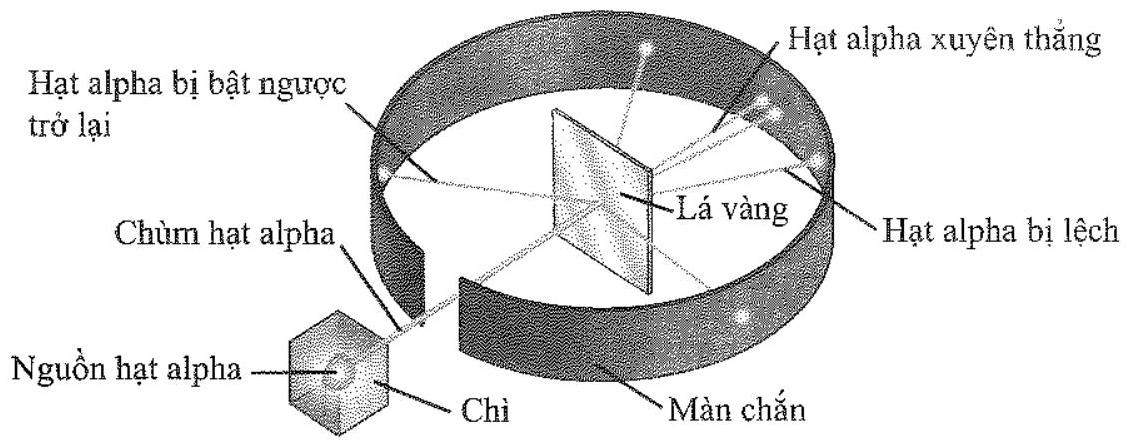
\includegraphics[max width=\textwidth, center]{2025_10_23_76620c17ffac1ae9b35bg-05}

Thí nghiệm bắn phá lá vàng bằng các hạt alpha của Rutherford

\section*{Bat \\
 3 NGUYÊN TỐ HOÁ HOC}
3.1. Đồng vị là những nguyên tử của cùng một nguyên tố hoá học, nhưng khác nhau về\\
A. tính chất hoá học.\\
B. khối lượng nguyên tử.\\
C. số proton.\\
D. số electron.\\
3.2. Trong tự nhiên, hydrogen có ba đồng vị $\left({ }_{1}^{1} \mathrm{H},{ }_{1}^{2} \mathrm{H},{ }_{1}^{3} \mathrm{H}\right)$. Nguyên tử khối trung bình của hydrogen bằng 1,008 . Hãy cho biết đồng vị nào của hydrogen chiếm tỉ lệ nhiều nhất trong tự nhiên.\\
A. ${ }_{1}^{1} \mathrm{H}$.\\
B. ${ }_{1}^{2} \mathrm{H}$.\\
C. ${ }_{1}^{3} \mathrm{H}$.\\
D. Không thể xác định được.\\
3.3. Hãy nối các mô tả trong cột A với các kí hiệu đồng vị ${ }_{\mathrm{Z}}^{\mathrm{A}} \mathrm{X}$ trong cột B cho phù hợp.

Côt A\\
a) Một đồng vị đồng có 34 neutron.\\
b) Một đồng vị đồng có 36 neutron.\\
c) Một đồng vị potassium có 21 neutron.\\
d) Một đồng vị argon có 22 neutron.

Côt B

\begin{enumerate}
  \item ${ }_{29}^{65} \mathrm{Cu}$
  \item ${ }_{29}^{63} \mathrm{Cu}$
  \item ${ }_{18}^{40} \mathrm{Ar}$
  \item ${ }_{19}^{40} \mathrm{~K}$
  \item ${ }_{18}^{40} \mathrm{~K}$\\
3.4. Cặp nguyên tử nào sau đây có cùng số neutron?\\
A. ${ }_{5}^{11} \mathrm{~B}$ và ${ }_{6}^{12} \mathrm{C}$.\\
B. ${ }_{3}^{7} \mathrm{Li}$ và ${ }_{4}^{9} \mathrm{Be}$.\\
C. ${ }_{12}^{24} \mathrm{Mg}$ và ${ }_{14}^{28} \mathrm{Si}$.\\
D. ${ }_{7}^{14} \mathrm{~N}$ và ${ }_{8}^{16} \mathrm{O}$.\\
3.5. Deuterium (D) là một đồng vị của hydrogen, được ứng dụng trong các lĩnh vực hạt nhân. Ion nào sau đây có số electron nhiều hơn số proton và số proton nhiều hơn số neutron (Biết $\mathrm{H}={ }_{1}^{1} \mathrm{H}, \mathrm{D}={ }_{1}^{2} \mathrm{H}, \mathrm{O}={ }_{8}^{16} \mathrm{O}$ )?\\
A. $\mathrm{D}^{-}$.\\
B. $\mathrm{H}_{3} \mathrm{O}^{+}$.\\
C. $\mathrm{OD}^{-}$.\\
D. $\mathrm{OH}^{-}$.\\
3.6. Phổ khối lượng của một mẫu lithium cho thấy nó chứa hai đồng vị là ${ }^{6} \mathrm{Li}$ và ${ }^{7} \mathrm{Li}$ với tỉ lệ phần trăm số nguyên tử mỗi đồng vị lần lượt là $7,42 \%$ và $92,58 \%$. Nguyên tử khối trung bình của mẫu lithium này (kết quả tính đến hai chữ số thập phân) là\\
A. 6,07 .\\
B. 6,50 .\\
C. 6,90 .\\
D. 6,93 .\\
3.7. Neon có ba đồng vị bền trong tự nhiên. Tỉ lệ phần trăm số nguyên tử mỗi đồng vị được thể hiện trong bảng sau:
\end{enumerate}

\begin{center}
\begin{tabular}{|l|c|c|c|}
\hline
Só khôl & A & 21 & 22 \\
\hline
Tilè $(\%)$ & 90,9 & 0,3 & 8,8 \\
\hline
\end{tabular}
\end{center}

Biết rằng nguyên tữ khối trung bình của Ne là 20,18 . Giá trị số khối A của đồng vị đầu tiên là\\
A. 19,00 .\\
B. 20,00 .\\
C. 20,01 .\\
D. Không xác định được.\\
3.8. Trong tự nhiên, carbon có hai đồng vị bền là ${ }^{12} \mathrm{C}$ và ${ }^{13} \mathrm{C}$; oxygen có ba đồng vị bền là ${ }^{16} \mathrm{O},{ }^{17} \mathrm{O}$ và ${ }^{18} \mathrm{O}$. Số lượng tối đa loại phân tử $\mathrm{CO}_{2}$ có thể tạo ra từ các đồng vị này là\\
A. 6 .\\
B. 9 .\\
C. 12 .\\
D. Vô số.\\
3.9. Phổ khối lượng của zirconium được biểu diễn như hình sau đây (điện tích z của các ion đồng vị zirconium đều bằng $1+$ ).\\
Số lượng đồng vị bền và nguyên tử khối trung bình của zirconium là:\\
A. 5 đồng vị, nguyên tử khối trung bình bằng 92,60 .\\
B. 5 đồng vị, nguyên tử khối trung bình bằng 91,32 .\\
C. 4 đồng vị, nguyên tử khối trung bình bằng 91,18 .\\
D. 4 đồng vị, nguyên tử khối trung bình bằng 92,00 .

\begin{figure}[h]
\begin{center}
  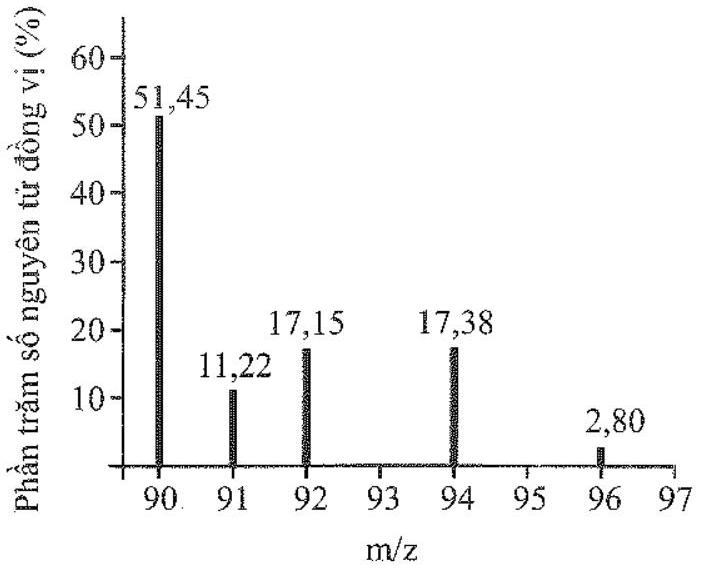
\includegraphics[width=\textwidth]{2025_10_23_76620c17ffac1ae9b35bg-07(4)}
\captionsetup{labelformat=empty}
\caption{Phổ khối lượng của zirconium}
\end{center}
\end{figure}

3.10*. Bạc có hai đồng vị bền trong tự nhiên: ${ }^{107} \mathrm{Ag}$ có hàm lượng tương đối là $51,8 \% ;{ }^{109} \mathrm{Ag}$ có hàm lượng tương đối là $48,2 \%$. Hãy vẽ phổ khối lượng của bạc và tính nguyên tử khối trung bình của Ag .\\
3.11*. Đồng có hai đồng vị bền trong tự nhiên là ${ }^{63} \mathrm{Cu}$ và ${ }^{65} \mathrm{Cu}$. Nguyên tử khối trung bình của đồng là 63,55 (điện tích z của các ion đồng vị đồng đều bằng $1+$ ). Hình vẽ phổ khối nào dưới đây là đúng?

\begin{figure}[h]
\begin{center}
  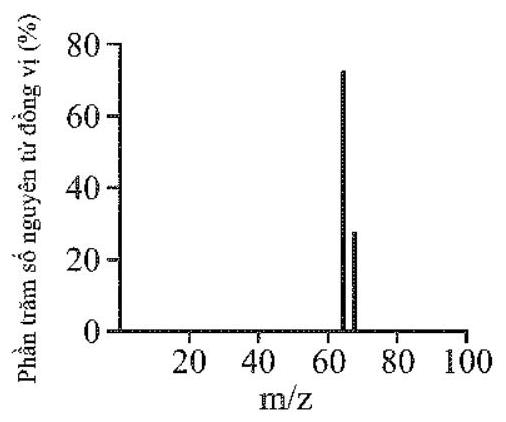
\includegraphics[width=\textwidth]{2025_10_23_76620c17ffac1ae9b35bg-07(2)}
\captionsetup{labelformat=empty}
\caption{(A)}
\end{center}
\end{figure}

\begin{figure}[h]
\begin{center}
  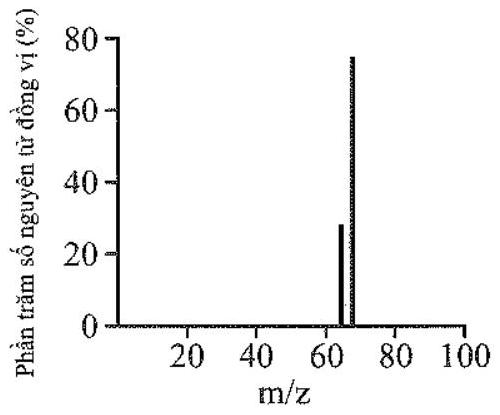
\includegraphics[width=\textwidth]{2025_10_23_76620c17ffac1ae9b35bg-07}
\captionsetup{labelformat=empty}
\caption{(C)}
\end{center}
\end{figure}

\begin{figure}[h]
\begin{center}
  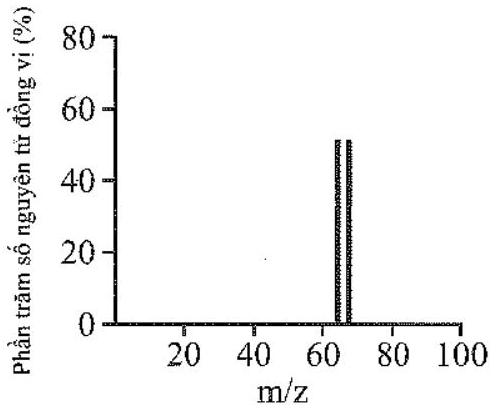
\includegraphics[width=\textwidth]{2025_10_23_76620c17ffac1ae9b35bg-07(1)}
\captionsetup{labelformat=empty}
\caption{(B)}
\end{center}
\end{figure}

\begin{figure}[h]
\begin{center}
  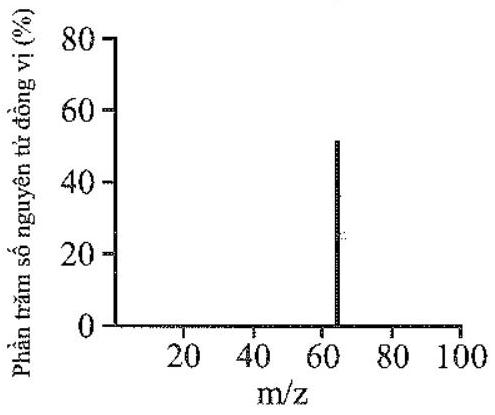
\includegraphics[width=\textwidth]{2025_10_23_76620c17ffac1ae9b35bg-07(3)}
\captionsetup{labelformat=empty}
\caption{(D)}
\end{center}
\end{figure}

3.12*. Đồng vị được sử dụng rộng rãi để nghiên cứu phản ứng hoá học. Cho biết vai trò của D (đồng vị ${ }_{1}^{2} \mathrm{H}$ ) và T (đồng vị ${ }_{1}^{3} \mathrm{H}$ ) là như nhau trong các phản ứng hoá học. Trong điều kiện thích hợp, xảy ra phản ứng sau:


\begin{equation*}
\mathrm{CH}_{2}=\mathrm{CH}-\mathrm{CH}_{2}-\mathrm{CH}_{2}-\mathrm{CH}=\mathrm{CHD} \rightleftharpoons \mathrm{CH}_{2}=\mathrm{CH}-\mathrm{CH}_{2}-\mathrm{CHD}-\mathrm{CH}=\mathrm{CH}_{2} \tag{1}
\end{equation*}


Vậy cũng trong điều kiện đó, phản ứng sau đây có xảy ra hay không?


\begin{equation*}
\mathrm{CD}_{2}=\mathrm{CD}-\mathrm{CD}_{2}-\mathrm{CD}_{2}-\mathrm{CD}=\mathrm{CDT} \rightleftharpoons \mathrm{CD}_{2}=\mathrm{CD}-\mathrm{CD}_{2}-\mathrm{CDT}-\mathrm{CD}=\mathrm{CD}_{2} \tag{2}
\end{equation*}


\section*{Bet \\
 $A$ MÔ HİNH NGUYÊN TỬ VÀ ORBITAL NGUYÊN TỬ}
4.1. Dựa vào mô hình nguyên tử Rutherford - Bohr, hãy cho biết phát biểu nào sau đây là đúng.\\
A. Số lượng electron tối đa trên các lớp là như nhau.\\
B. Năng lượng của các electron trên các lớp khác nhau có thể bằng nhau.\\
C. Khi quay quanh hạt nhân theo một quỹ đạo xác định, năng lượng của electron là không đổi.\\
D. Electron ở gần hạt nhân nhất có năng lượng cao nhất.\\
4.2. Theo mô hình Rutherford - Bohr, khi một nguyên tử H hấp thụ một năng lượng đủ lớn, electron sẽ\\
A. chuyển từ lớp electron gần hạt nhân sang lớp xa hạt nhân hơn.\\
B. chuyển từ lớp electron xa hạt nhân về lớp gần hạt nhân hơn.\\
C. không thay đổi trạng thái.\\
D. có thể chuyển sang lớp khác bất kì.\\
4.3. Phát biểu nào sau đây không đúng khi nói về mô hình Rutherford - Bohr?\\
A. Electron trên lớp K có năng lượng cao hơn trên lớp L .\\
B. Electron trên lớp M có năng lượng cao hơn trên lớp K .\\
C. Electron ở lớp K gần hạt nhân hơn so với electron ở lớp L .\\
D. Electron ở lớp M xa hạt nhân hơn so với electron ở lớp L .\\
4.4. Nguyên tử F có 9 electron. Theo mô hình Rutherford - Bohr, tỉ lệ số lượng electron trên lớp thứ hai so với số lượng electron trên lớp thứ nhất là\\
A. $2: 12$.\\
B. $7: 2$.\\
C. $5: 2$.\\
D. $2: 7$.\\
4.5. Điền từ/ cụm từ thích hợp vào chỗ trống trong mô tả sau đây về mô hình hành tinh nguyên tử theo Rutherford - Bohr.\\
Khối lượng nguyên tử tập trung ở ...(1)... Electron quay xung quanh hạt nhân theo những ...(2)... xác định. Electron ở càng xa hạt nhân thì có năng lượng càng ...(3)... Khi nguyên tử hấp thụ năng lượng phù hợp, electron sẽ chuyển ...(4)... hạt nhân hơn.\\
4.6. Nguyên tử $O$ có 8 electron. Theo mô hình Rutherford - Bohr, nguyển tử $O$ có số electron có cùng năng lượng ở lớp thứ nhất là\\
A. 2 .\\
B. 4 .\\
C. 6 .\\
D. 8 .\\
4.7. Theo mô hình nguyên tử hiện đại, xác suất tìm thấy electron lớn nhất là ở\\
A. bên ngoài các orbital nguyên tử.\\
B. trong các orbital nguyên tử.\\
C. bên trong hạt nhân nguyên tử.\\
D. bất kì vị trí nào trong không gian.\\
4.8. Vùng nào sau đây ứng với xác suất tìm thấy electron trong nguyên tử bằng $100 \%$ ?\\
A. Bên ngoài các orbital nguyên tử.\\
B. Trong các orbital nguyên tử.\\
C. Trong toàn bộ khoảng không gian xung quanh hạt nhân.\\
D. Ở bên trong hạt nhân.\\
4.9. Mỗi phát biểu sau đây về mô hình nguyên tử hiện đại là đúng hay sai?\\
(1) Theo mô hình nguyên tử hiện đại, electron chuyển động không theo những quỹ đạo xác định trong cả khu vực không gian xung quanh hạt nhân.\\
(2) Tất cả các AO nguyên tử đều có hình dạng giống nhau.\\
(3) Mỗi AO nguyên tử chỉ có thể chứa được 1 electron.\\
(4) Các electron s chuyển động trong các AO có hình số tám nổi.\\
4.10. Hình ảnh bên mô tả $A O p$ với hai thuỳ. Những phát biểu nào sau đây là đúng?\\
A. Xác suất tìm thấy electron ở mỗi thuỳ là khoảng $45 \%$.\\
B. Xác suất tìm thấy electron ở mỗi thuỳ là khoảng $90 \%$.\\
C. Xác suất tìm thấy electron trong AO p là khoảng $90 \%$.\\
D. Xác suất tìm thấy electron trong AO p là khoảng $45 \%$.

\begin{figure}[h]
\begin{center}
  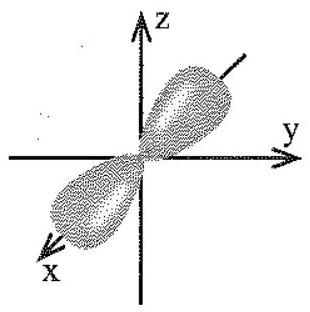
\includegraphics[width=\textwidth]{2025_10_23_76620c17ffac1ae9b35bg-09}
\captionsetup{labelformat=empty}
\caption{AO p}
\end{center}
\end{figure}

4.11. Nếu 5 electron được điền vào 3 AO thì số lượng electron độc thân là\\
A. 0 .\\
B. 1 .\\
C. 2 .\\
D. 5 .\\
4.12. Fluorine là nguyên tố hoá học có mặt trong nhiều hợp chất được ứng dụng trong nha khoa, y tế. Nguyên tử F có 9 electron. Hãy đề xuất phương án sắp xếp những electron này vào 5 orbital nguyên tử. Cho biết số cặp electron ghép đôi và số lượng electron độc thân trong trường hợp đó.\\
4.13. Cần ît nhất bao nhiêu orbital nguyên tữ để chứa được: $2,8,18$ electron?\\
4.14*. Theo mô hình Rutherford - Bohr, electron trong nguyên tử hydrogen chuyển động trên các quỹ đạo xác định xung quanh tâm là hạt nhân nguyên tử. Mỗi quỹ đạo được đặc trưng bởi một giá trị $\mathrm{n}(\mathrm{n}=1,2,3, \ldots)$. Giá trị của n cũng chính là số thứ tự của lớp electron. Bán kính của quỹ đạo thứ n (kí hiệu là $\mathrm{r}_{\mathrm{n}}$ ) của nguyên tử hydrogen có thể tính theo công thức: $\mathrm{r}_{\mathrm{n}}=\mathrm{n}^{2} \times 0,529(\AA)$. Hãy tính bán kính quỹ đạo thứ nhất và thứ hai (tương ứng với $\mathrm{n}=1$ và $\mathrm{n}=2$ ) của nguyên tử hydrogen.\\
4.15*. Bán kính của quỹ đạo thứ $n\left(r_{n}\right)$ của các ion chỉ chứa 1 electron như $\mathrm{He}^{+}$, $\mathrm{Li}^{2+}, \mathrm{Be}^{3+}$ có thể tính theo công thức:

$$
r_{n}=n^{2} \times \frac{0,529}{Z^{2}}(\AA), \text { trong đó } Z \text { là điện tích hạt nhân. }
$$

Hãy so sánh (có giải thích) bán kính quỹ đạo thứ nhất của các ion $\mathrm{He}^{+}, \mathrm{Li}^{2+}, \mathrm{Be}^{3+}$.\\
4.16*. Năng lượng của electron trong hệ gồm 1 electron và 1 hạt nhân (như H , $\mathrm{He}^{+}, \ldots$ ) theo mô hình Rutherford - Bohr cũng như mô hình hiện đại đều phụ thuộc vào số thứ tự của lớp (n) và điện tích hạt nhân (Z) như sau:

$$
E_{n}=-2,18 \times 10^{-18} \times \frac{Z^{2}}{n^{2}}(J)
$$

trong đó Z là điện tích hạt nhân; $\mathrm{n}=1,2,3, \ldots$ là số thứ tự của lớp electron. Hãy tính và so sánh (có giải thích) năng lượng của electron ở lớp thứ nhất của $\mathrm{H}, \mathrm{He}^{+}, \mathrm{Li}^{2+}$.

\section*{101 \\
 5 LỚP, PHÂN LỚP VÀ CẤU HÌNH ELECTRON}
5.1. Phát biểu nào sau đây là đúng?\\
A. Electron trong cùng một lớp có năng lượng bằng nhau.\\
B. Electron trong cùng một phân lớp có năng lượng bằng nhau.\\
C. Electron ở các phân lớp $1 \mathrm{~s}, 2 \mathrm{~s}, 3 \mathrm{~s}$ có năng lượng bằng nhau.\\
D. Electron ở lớp bên ngoài có năng lượng thấp hơn electron ở lớp bên trong.\\
5.2. Phát biểu nào sau đây không đúng?\\
A. Electron càng ở xa hạt nhân thì có năng lượng càng thấp.\\
B. Số lượng electron tối đa trong một phân lớp luôn là một số chẵn.\\
C. Phân lớp p có nhiều orbital hơn phân lớp s .\\
D. Số electron tối đa trên phân lớp p gấp ba lần số electron tối đa trên phân lớp s.\\
5.3. Mỗi phát biểu sau đây là đúng hay sai?\\
(1) Số lượng orbital trong các phân lớp $1 \mathrm{~s}, 2 \mathrm{~s}, 3 \mathrm{~s}$ là bằng nhau.\\
(2) Số lượng orbital trong các phân lớp $3 \mathrm{~s}, 3 \mathrm{p}, 3 \mathrm{~d}$ là bằng nhau.\\
(3) Các electron trên các phân lớp $1 \mathrm{~s}, 2 \mathrm{~s}, 3 \mathrm{~s}$ có năng lượng bằng nhau.\\
(4) Các electron trên các phân lớp $3 \mathrm{~s}, 3 \mathrm{p}, 3 \mathrm{~d}$ có năng lượng bằng nhau.\\
(5) Số lượng electron tối đa trong một lớp là $2 n^{2}$.\\
(6) Số lượng các orbital trong một phân lớp ( $\mathrm{s}, \mathrm{p}, \mathrm{d}, \mathrm{f}$ ) luôn là một số lẻ.\\
5.4. Điền từ/ cựm từ hoặc số thích hợp vào chỗ trống trong mỗi phát biểu sau:\\
a) Các electron trong lớp vỏ nguyên tử được phân bố vào các ...(1)... và ...(2)... dựa theo năng lượng của chúng. Các electron thuộc cùng một lớp có năng lượng ...(3)..., các electron thuộc cùng một phân lớp có năng lượng ...(4).... Các electron ở ...(5)... có vai trò quyết định đến tính chất hoá học đặc trưng của nguyên tố.\\
b) Magnesium được sử dụng nhiều trong công nghiệp để chế tạo các bộ phận của máy bay, ô tô. Nguyên tử magnesium có 12 electron, được phân bố vào ...(1)... lớp. Lớp ngoài cùng của magnesium có ...(2)... electron.\\
5.5. Số phân lớp bão hoà trong các phân lớp: $1 \mathrm{~s}^{2}, 2 \mathrm{~s}^{2}, 2 \mathrm{p}^{3}, 3 \mathrm{~d}^{10}, 3 \mathrm{p}^{4}$ là\\
A. 1 .\\
B. 2 .\\
C. 3 .\\
D. 5 .\\
5.6. Ghép mỗi biểu diễn ô orbital của phân lớp p ở cột A với mô tả thích hợp ở cột B .

Cột A\\
a)\\
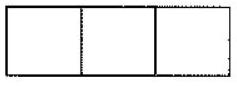
\includegraphics[max width=\textwidth, center]{2025_10_23_76620c17ffac1ae9b35bg-11(2)}\\
b)\\
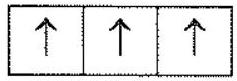
\includegraphics[max width=\textwidth, center]{2025_10_23_76620c17ffac1ae9b35bg-11(1)}\\
c)\\
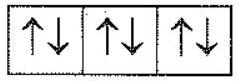
\includegraphics[max width=\textwidth, center]{2025_10_23_76620c17ffac1ae9b35bg-11}

\section*{Cột B}
\begin{enumerate}
  \item Phân lớp bão hoà
  \item Phân lớp bán (nửa) bão hoà
  \item Phân lớp chứa các AO trống\\
5.7. Nguyên tử O có 8 electron. Biểu diễn sự sắp xếp electron trong nguyên tử O theo orbital nào sau đây là đúng?\\
1s
\end{enumerate}

\begin{figure}[h]
\begin{center}
\captionsetup{labelformat=empty}
\caption{A.}
  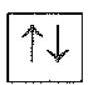
\includegraphics[width=\textwidth]{2025_10_23_76620c17ffac1ae9b35bg-12}
\end{center}
\end{figure}

3s\\
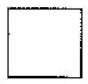
\includegraphics[max width=\textwidth, center]{2025_10_23_76620c17ffac1ae9b35bg-12(6)}\\
B.\\
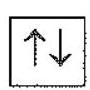
\includegraphics[max width=\textwidth, center]{2025_10_23_76620c17ffac1ae9b35bg-12(2)}\\
2 s

\begin{figure}[h]
\begin{center}
\captionsetup{labelformat=empty}
\caption{A.}
  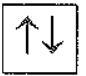
\includegraphics[width=\textwidth]{2025_10_23_76620c17ffac1ae9b35bg-12(1)}
\end{center}
\end{figure}

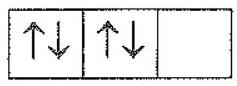
\includegraphics[max width=\textwidth, center]{2025_10_23_76620c17ffac1ae9b35bg-12(11)}\\
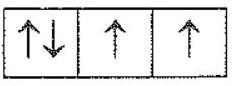
\includegraphics[max width=\textwidth, center]{2025_10_23_76620c17ffac1ae9b35bg-12(13)}\\
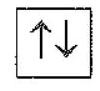
\includegraphics[max width=\textwidth, center]{2025_10_23_76620c17ffac1ae9b35bg-12(8)}\\
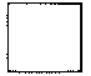
\includegraphics[max width=\textwidth, center]{2025_10_23_76620c17ffac1ae9b35bg-12(14)}\\
C.\\
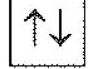
\includegraphics[max width=\textwidth, center]{2025_10_23_76620c17ffac1ae9b35bg-12(7)}\\
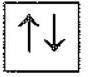
\includegraphics[max width=\textwidth, center]{2025_10_23_76620c17ffac1ae9b35bg-12(10)}\\
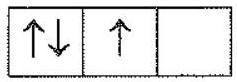
\includegraphics[max width=\textwidth, center]{2025_10_23_76620c17ffac1ae9b35bg-12(9)}\\
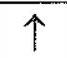
\includegraphics[max width=\textwidth, center]{2025_10_23_76620c17ffac1ae9b35bg-12(12)}\\
D.\\
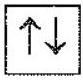
\includegraphics[max width=\textwidth, center]{2025_10_23_76620c17ffac1ae9b35bg-12(4)}\\
$\uparrow \downarrow$\\
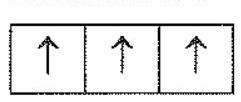
\includegraphics[max width=\textwidth, center]{2025_10_23_76620c17ffac1ae9b35bg-12(3)}\\
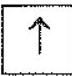
\includegraphics[max width=\textwidth, center]{2025_10_23_76620c17ffac1ae9b35bg-12(5)}\\
5.8. Các nguyên tử $\mathrm{Ne}, \mathrm{Na}$ và F có Z lần lượt là 10,11 và 9 . Cấu hình electron của $\mathrm{Ne}, \mathrm{Na}^{+}$và $\mathrm{F}^{-}$tương ứng là:\\
A. $1 s^{2} 2 s^{2} 2 p^{6} ; 1 s^{2} 2 s^{2} 2 p^{6} 3 s^{1}$ và $1 s^{2} 2 s^{2} 2 p^{5}$.\\
B. đều có cấu hình $1 \mathrm{~s}^{2} 2 \mathrm{~s}^{2} 2 \mathrm{p}^{6}$.\\
C. $1 s^{2} 2 s^{2} 2 p^{6} ; 1 s^{2} 2 s^{2} 2 p^{5}$ và $1 s^{2} 2 s^{2} 2 p^{4}$.\\
D. $1 s^{2} 2 s^{2} 2 p^{6} ; 1 s^{2} 2 s^{2} 2 p^{5}$ và $1 s^{1} 2 s^{2} 2 p^{3}$.\\
5.9. Biết rằng điện tích hạt nhân của $\mathrm{C}, \mathrm{N}, \mathrm{O}$ và F lần lượt là $6,7,8$ và 9 . Ghép mỗi cấu hình electron ở cột A với nguyên tử/ ion thích hợp ở cột B .

\section*{Cột A}
a) $1 s^{2} 2 s^{2}$\\
b) $1 s^{2} 2 s^{2} 2 p^{4}$\\
c) $1 s^{2} 2 s^{2} 2 p^{5}$\\
d) $1 s^{2} 2 s^{2} 2 p^{6}$

\section*{Cột B}
1.O\\
2. $\mathrm{C}^{2+}$\\
3. $\mathrm{N}^{3-}$\\
4. F\\
5. $\mathrm{C}^{2-}$\\
5.10. Trong các nguyên tử $N(Z=7), O(Z=8), F(Z=9)$ và $N e(Z=10)$, nguyên tử có nhiều electron độc thân nhất là\\
A. N.\\
B. O.\\
C. F.\\
D. Ne.\\
5.11. Nối mỗi cấu hình electron của nguyên tử ở cột A với loại nguyên tố hoá học thích hợp ở cột B.

Cột A\\
a) $1 s^{2} 2 s^{2} 2 p^{6}$\\
b) $1 s^{2} 2 s^{2} 2 p^{5}$\\
c) $1 s^{2} 2 s^{2} 2 p^{6} 3 s^{1}$\\
d) $1 s^{2} 2 s^{2} 2 p^{6} 3 s^{2} 3 p^{3}$

\section*{Cột B}
\begin{enumerate}
  \item Kim loại
  \item Phi kim
  \item Khí hiếm\\
5.12. Cấu hình electron của một nguyên tử được biểu diễn dưới dạng các ô orbital như sau:\\
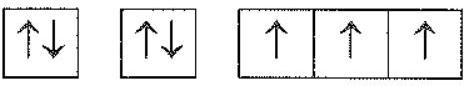
\includegraphics[max width=\textwidth, center]{2025_10_23_76620c17ffac1ae9b35bg-13}
\end{enumerate}

Số electron hoá trị và tính chất đặc trưng của nguyên tố hoá học này là\\
A. 3, tính kim loại.\\
B. 5, tính phi kim.\\
C. 7, tính phi kim.\\
D. 4, tính kim loại.\\
5.13. Cho các cấu hình electron của một số nguyên tử nguyên tố như sau:\\
(1) $1 s^{2} 2 s^{2} 2 p^{6}$\\
(2) $1 s^{2} 2 s^{2} 2 p^{6} 3 s^{2}$\\
(3) $1 s^{2} 2 s^{2} 2 p^{6} 3 s^{2} 3 p^{6} 3 d^{6} 4 s^{2}$\\
(4) $1 s^{2} 2 s^{2} 2 p^{6} 3 s^{2} 3 p^{6} 3 d^{1} 4 s^{2}$\\
(5) $1 s^{2} 2 s^{2} 2 p^{6} 3 s^{2} 3 p^{4}$\\
(6) $1 s^{2} 2 s^{2} 2 p^{6} 3 s^{2} 3 p^{5}$

Số lượng các nguyên tố kim loại trong số các nguyên tố ở trên là\\
A. 1 .\\
B. 2 .\\
C. 3 .\\
D. 4 .\\
5.14. Từ các nguyên tử có thể tạo ra các ion bằng cách thêm hoặc bớt electron từ nguyên tữ đó.\\
a) Oxygen là nguyên tố chiếm tỉ lệ phần trăm khối lượng cao nhất trong cơ thể con người (khoảng $65 \%$ ). Hãy viết cấu hình electron của O và $\mathrm{O}^{2-}(\mathrm{Z}=8)$. Cho biết để hình thành ion $\mathrm{O}^{2-}$, nguyên tử O sẽ nhận thêm electron vào orbital nào. Xác định số electron độc thân trong nguyên tử và ion này.\\
b) Nhôm (aluminium) được sử dụng phổ biến trong đời sống (chế tạo dụng cụ nhà bếp, cửa,...) cũng như trong công nghiệp (chế tạo một số bộ phận của máy bay). Hãy biểu diễn cấu hình electron của Al và ion $\mathrm{Al}^{3+}(\mathrm{Z}=13)$ dưới dạng ô orbital. Cho biết để tạo thành ion $\mathrm{Al}^{3+}$, nguyên tử Al sẽ mất đi electron từ orbital nào. Xác định số electron độc thân trong các nguyên tử và ion này.\\
5.15. Hãy cho biết những nguyên tử và ion (cation mang điện tích $1+, 2+$ hoặc anion mang điện tích $1-, 2-$ ) nào có cấu hình electron $1 s^{2} 2 s^{2} 2 p^{6}$.\\
5.16. Tại một khu vực của Úc, gia súc không phát triển mạnh mặc đù có thức ăn thô xanh thích hợp. Một cuộc điều tra cho thấy nguyên nhân là do không có đủ cobalt trong đất. Cobalt tạo thành cation ở hai dạng là $\mathrm{Co}^{2+}$ và $\mathrm{Co}^{3+}(\mathrm{Z}=27)$. Viết cấu hình electron của hai cation này và sơ đồ phân bố các electron vào các ô orbital. Cho biết số electron độc thân trong mỗi ion.\\
5.17. Bromine $(Z=35)$ dễ phản ứng, trong khi krypton $(Z=36)$ tương đối trơ về mặt hoá học. Giải thích sự khác biệt này dựa trên cấu hình electron của chúng.\\
5.18*. Cũng giống như nam châm, mỗi nguyên tử/ ion cũng có thể có từ tính (bị nam châm hút). Nếu nguyên tử/ ion có electron độc thân thì nó có từ tính và được gọi là chất thuận từ. Ngược lại, nguyên tử/ ion nếu không có electron độc thân thì được gọi là chất nghịch từ. Hãy giải thích vì sao nguyên tử Cu $(\mathrm{Z}=29)$ thuận từ nhưng ion $\mathrm{Cu}^{+}$lại nghịch từ.

\section*{CHỦ DỂ 2: BẢNG TUẦN HOÀN CÁC NGUYÊN TỐ HOÁ HỌC \\
 BTI CẤU TAO CỦA BẢNG TUẦN HOÀN CÁC NGUYÊN TỐ HOÁ HOC}
6.1. Chọn phương án đúng để hoàn thành các câu sau:\\
a) Mỗi nguyên tố hoá học được xếp vào một ...(1)... trong bảng tuần hoàn. Mỗi hàng trong bảng tuần hoàn được gọi là một ...(2)... Mỗi cột trong bảng tuần hoàn được gọi là một ...(3)...\\
A. (1) nhóm, (2) chu kì, (3) ô.\\
B. (1) ô, (2) chu kì, (3) nhóm.\\
C. (1) ô, (2) họ, (3) nhóm.\\
D. (1) ô, (2) chu kì, (3) nhóm chính.\\
b) Trong bảng tuần hoàn các nguyên tố hoá học do Mendeleev đề xuất, các nguyên tố được sắp xếp theo chiều tăng dần của ...(1).... Trong bảng tuần hoàn các nguyên tố hoá học hiện đại, các nguyên tố được sắp xếp theo chiều tăng dần của ...(2)....\\
A. (1) số electron hoá trị, (2) khối lượng nguyên tử.\\
B. (1) số hiệu nguyên tử, (2) khối lượng nguyên tử.\\
C. (1) khối lượng nguyên tử, (2) số hiệu nguyên tử.\\
D. (1) số electron hoá trị, (2) số hiệu nguyên tử.\\
6.2. Số hiệu nguyên tử của nguyên tố hoá học bằng\\
A. số thứ tự của ô nguyên tố.\\
B. số thứ tự của chu kì.\\
C. số thứ tự của nhóm.\\
D. số electron lớp ngoài cùng của nguyên tử.\\
6.3. Mỗi phát biểu sau đây về bảng tuần hoàn các nguyên tố hoá học là đúng hay sai?\\
(1) Số thứ tự của nhóm luôn luôn bằng số electron ở lớp vỏ ngoài cùng của nguyên tử nguyên tố thuộc nhóm đó.\\
(2) Số electron ở lớp vỏ ngoài cùng càng lớn thì số thứ tự của nhóm càng lớn.\\
(3) Nguyên tử các nguyên tố trong cùng một hàng có cùng số lớp electron.\\
(4) Nguyên tử các nguyên tố trong cùng một cột có cùng số electron hoá trị.\\
6.4. Hình bên mô tả ô nguyên tố của vàng trong bảng tuần hoàn các nguyên tố hoá học.\\
Những thông tin thu được từ ô nguyên tố này là:\\
A. Vàng có kí hiệu là Au , nguyên tử có 79 proton, nguyên tử khối trung bình là 196,97 .\\
B. Vàng và các hợp chất của vàng có kí hiệu là Au , có số hiệu nguyên tử là 79 , nguyên tử khối trung bình là 196,97 .\\
C. Vàng và các hợp chất của vàng có kí hiệu là Au , có số hiệu nguyên tử là 79 , vàng có hai đồng vị với số khối là 196 và 197.\\
D. Vàng có kí hiệu là Au , số hiệu nguyên tử là 79 , có hai đồng vị với số khối là 196 và 197.\\
6.5. Cấu hình electron của nguyên tử oxygen là $1 s^{2} 2 s^{2} 2 p^{4}$. Vị trí của oxygen trong bảng tuần hoàn là:\\
A. ô số 6, chu kì 2, nhóm VIA.\\
B. ô số 6 , chu kì 3 , nhóm VIB.\\
C. ô số 8, chu kì 2, nhóm VIA.\\
D. ô số 8 , chu kì 2 , nhóm VIB.\\
6.6. Cấu hình electron của nguyên tử sắt là $1 s^{2} 2 s^{2} 2 p^{6} 3 s^{2} 3 p^{6} 3 d^{6} 4 s^{2}$. Vị trí của sắt trong bảng tuần hoàn là:\\
A. ô số 26 , chu kì 3 , nhóm VIIIB.\\
B. ô số 26 , chu kì 3 , nhóm VIIIA.\\
C. ô số 26, chu kì 4, nhóm VIIIA.\\
D. ô số 26 , chu kì 4 , nhóm VIIIB.\\
6.7. Cấu hình electron của fluorine là $1 s^{2} 2 s^{2} 2 p^{5}$, của chlorine là $1 s^{2} 2 s^{2} 2 p^{6} 3 s^{2} 3 p^{5}$. Những phát biểu nào sau đây là đúng?\\
A. F và Cl nằm ở cùng một nhóm.\\
B. F và Cl có số electron lớp ngoài cùng bằng nhau.\\
$\mathrm{C} . \mathrm{F}$ và Cl có số electron lớp ngoài cùng khác nhau.\\
D. F và Cl nằm ở cùng một chu kì.\\
E. Số thứ tự chu kì của Cl lớn hơn F .

G . Cl là nguyên tố nhóm $\mathrm{B}, \mathrm{F}$ là nguyên tố nhóm A .\\
6.8. Hãy ghép mỗi cấu hình electron ở cột A với mô tả thích hợp về vị trí nguyên tố trong bảng tuần hoàn ở cột B .

\section*{Côt $\mathbf{A}$}
a) $1 s^{2} 2 s^{2} 2 p^{6}$\\
b) $[\mathrm{Ar}] 3 \mathrm{~d}^{5} 4 \mathrm{~s}^{1}$\\
c) $[\mathrm{He}] 2 s^{2} 2 p^{1}$\\
d) $1 s^{2} 2 s^{2} 2 p^{6} 3 s^{1}$

\section*{Cột B}
\begin{enumerate}
  \item Nguyên tố nhóm IIIA
  \item Nguyên tố ở ô thứ 11
  \item Nguyên tố nhóm VIIIA
  \item Nguyên tố chu kì 4\\
6.9. Cho cấu hình electron các nguyên tố sau đây: $\mathrm{Na}:[\mathrm{Ne}] 3 \mathrm{~s}^{1}, \mathrm{Cr}:[\mathrm{Ar}] 3 \mathrm{~d}^{5} 4 \mathrm{~s}^{1}$, $\mathrm{Br}:[\mathrm{Ar}] 3 \mathrm{~d}^{10} 4 \mathrm{~s}^{2} 4 \mathrm{p}^{5}, \mathrm{~F}: 1 \mathrm{~s}^{2} 2 \mathrm{~s}^{2} 2 \mathrm{p}^{5}, \mathrm{Cu}:[\mathrm{Ar}] 3 \mathrm{~d}^{10} 4 \mathrm{~s}^{1}$. Số nguyên tố thuộc khối s, $\mathrm{p}, \mathrm{d}$ trong các nguyên tố trên lần lượt là:\\
A. $2,1,2$.\\
B. 1, 2, 2 .\\
C. $1,1,3$.\\
D. Không xác định được.\\
6.10. Những nguyên tố được xếp riêng bên dưới bảng tuần hoàn thuộc khối nguyên tố nào?\\
A. s.\\
B. p.\\
C. d.\\
D. f.\\
6.11. Hãy giải thích vì sao khối nguyên tố s trong bảng tuần hoàn chỉ có hai cột trong khi khối nguyên tố p có sáu cột.\\
6.12. Vì sao số lượng các nguyên tố trong các chu kì của bảng tuần hoàn có sự khác biệt: chu kì 1 có 2 nguyên tố; mỗi chu kì 2 và 3 có 8 nguyên tố; chu kì 4 có 18 nguyên tố?\\
6.13. Calcium (Ca) là nguyên tố kim loại chiếm khối lượng nhiều nhất trong cơ thể con người. Răng và xương là các bộ phận chứa nhiều calcium nhất. Số hiệu nguyên tử của Ca là 20 . Hãy xác định vị trí của calcium trong bảng tuần hoàn.\\
6.14. Em cần giải một mật mã sử dụng các kí hiệu nguyên tố để xác định các chữ cái trong mật mã. Quy tắc của mật mã như sau:\\
(1) Cho một dãy số, trong đó mỗi số là tổng của số hiệu nguyên tử và số lớp electron của một nguyên tử ứng với một nguyên tố hoá học.\\
(2) Chữ cái đầu tiên trong kí hiệu hoá học của mỗi nguyên tố thu được từ việc giải mã dãy số ở quy tắc thứ nhất sẽ tương ứng với một chữ cái trong mật mã. Em hãy thử giải mật mã theo quy tắc trên với dãy số sau: $8,2,69,29,58,19$, $26,42,76$ (các chữ cái của mật mã sắp xếp theo đúng thứ tự tương ứng với các con số).
\end{enumerate}

\section*{BM XU HƯỚNG BIẾN DỔI MÔT SỐ TÍNH CHẤT \\
 1 CỦA ĐỚN CHẤT, BIẾN ĐỔI THÀNH PHẦN VÀ TÍNH CHẤT CỦA HỢ PCHẤT TRONG MỘT CHU KÌ VÀ TRONG MỘT NHÓM}
7.1. Chọn nguyên tử có bán kính lớn hơn trong mỗi cặp nguyên tử nguyên tố sau.\\
a) Al và In.\\
b) Si và N .\\
c) P và Pb .\\
d) C và F .\\
7.2. Dãy nguyên tử nào sau đây có bán kính tăng dần?\\
A. $\mathrm{F}<\mathrm{S}<\mathrm{Si}<\mathrm{Ge}<\mathrm{Ca}<\mathrm{Rb}$.\\
B. $\mathrm{F}<\mathrm{Si}<\mathrm{S}<\mathrm{Ca}<\mathrm{Ge}<\mathrm{Rb}$.\\
C. $\mathrm{Rb}<\mathrm{Ca}<\mathrm{Ge}<\mathrm{Si}<\mathrm{S}<\mathrm{F}$.\\
D. $\mathrm{F}<\mathrm{Si}<\mathrm{S}<\mathrm{Ge}<\mathrm{Ca}<\mathrm{Rb}$.\\
7.3. Dãy các ion nào sau đây có bán kính tăng dần?\\
A. $\mathrm{S}^{2-}<\mathrm{Cl}^{-}<\mathrm{K}^{+}<\mathrm{Ca}^{2+}$.\\
B. $\mathrm{K}^{+}<\mathrm{Ca}^{2+}<\mathrm{S}^{2-}<\mathrm{Cl}^{-}$.\\
C. $\mathrm{Cl}^{-}<\mathrm{S}^{2-}<\mathrm{Ca}^{2+}<\mathrm{K}^{+}$.\\
D. $\mathrm{Ca}^{2+}<\mathrm{K}^{+}<\mathrm{Cl}^{-}<\mathrm{S}^{2-}$.\\
7.4. Cho bảng số liệu sau đây:

\begin{center}
\begin{tabular}{|l|l|l|l|}
\hline
Nguyên tú & Bán kinh (pm) & Ion & Bán kính (pm) \\
\hline
Na & 186 & $\mathrm{Na}^{+}$ & 98 \\
\hline
K & 227 & $\mathrm{K}^{+}$ & ? \\
\hline
\end{tabular}
\end{center}

Dựa trên xu hướng biến đổi tuần hoàn và dữ liệu trong bảng trên, giá trị nào sau đây là phù hợp nhất đối với bán kính ion $\mathrm{K}^{+}$?\\
A. 90 pm .\\
B. 133 pm .\\
C. 195 pm .\\
D. 295 pm .\\
7.5. Phát biểu nào sau đây là đúng về xu hướng biến đổi tính kim loại trong bảng tuần hoàn các nguyên tố hoá học?\\
A. Tính kim loại của các nguyên tố tăng theo chiều từ trái sang phải trong một chu kì và từ trên xuống dưới trong một nhóm.\\
B. Tính kim loại giảm dần theo chiều từ trái sang phải trong một chu kì và tăng dần từ trên xuống dưới trong một nhóm.\\
C. Tính kim loại giảm dần theo chiều từ trái sang phải trong một chu kì và từ trên xuống dưới trong một nhóm.\\
D. Tính kim loại tăng dần theo chiều từ trái sang phải trong một chu kì và giảm dần từ trên xuống dưới trong một nhóm.\\
7.6. Chọn nguyên tố thể hiện tính kim loại nhiều hơn trong mỗi cặp nguyên tố sau:\\
a) Sr và Sb .\\
b) As và Bi.\\
c) B và O .\\
d) S và As .\\
7.7. Dãy các nguyên tố nào sau đây có tính kim loại giảm dần?\\
A. $\mathrm{Sr}>\mathrm{Al}>\mathrm{P}>\mathrm{Si}>\mathrm{N}$.\\
B. $\mathrm{Sr}>\mathrm{Al}>\mathrm{P}>\mathrm{N}>\mathrm{Si}$.\\
C. $\mathrm{Sr}>\mathrm{Al}>\mathrm{Si}>\mathrm{P}>\mathrm{N}$.\\
D. $\mathrm{Sr}>\mathrm{Si}>\mathrm{Al}>\mathrm{P}>\mathrm{N}$.\\
7.8. Xu hướng biến đổi độ âm điện của các nguyên tố trong bảng tuần hoàn tương tự như xu hướng biến đồi của yếu tố nào sau đây?\\
(1) Tính kim loại.\\
(2) Tính phi kim.\\
(3) Bán kính nguyên tử.\\
A. (1).\\
B. (2).\\
C. (3).\\
D. (1), (2) và (3).\\
7.9. Cấu hình electron nào sau đây ứng với nguyên tố có độ âm điện lớn nhất?\\
A. $1 s^{2} 2 s^{2} 2 p^{5}$.\\
B. $1 \mathrm{~s}^{2} 2 \mathrm{~s}^{2} 2 \mathrm{p}^{6}$.\\
C. $1 s^{2} 2 s^{2} 2 p^{6} 3 s^{1}$.\\
D. $1 s^{2} 2 s^{2} 2 p^{6} 3 s^{2} 3 p^{2}$.\\
7.10. Điền kí hiệu hoá học hoặc cụm từ thích hợp vào chỗ trống trong đoạn thông tin sau:\\
Trong số các nguyên tố thuộc chu kì 2 trong bảng tuần hoàn (trừ Ne), ...(1)... là nguyên tố có độ âm điện nhỏ nhất và bán kính nguyên tử ...(2)...; ...(3)... là nguyên tố có độ âm điện lớn nhất nhưng bán kính nguyên tử ...(4)... Tính kim loại giảm dần từ ...(5)... tới ...(6)..., còn tính phi kim thì biến đổi theo chiều ngược lại.\\
7.11. Trong liên kết $\mathrm{H}-\mathrm{X}$ (với X là $\mathrm{F}, \mathrm{Cl}, \mathrm{Br}$ ), cặp electron trong liên kết sẽ bị lệch về nguyên tử X do chúng có độ âm điện lớn hơn H . Hãy sắp xếp các nguyên tử X theo chiều giảm dần mức độ lệch của cặp electron liên kết về phía nó.\\
A. $\mathrm{Br}>\mathrm{Cl}>\mathrm{F}$.\\
B. $\mathrm{Cl}>\mathrm{F}>\mathrm{Br}$.\\
C. $\mathrm{F}>\mathrm{Cl}>\mathrm{Br}$.\\
D. Mức độ lệch của cặp electron là như nhau trong ba trường hợp.\\
7.12. Phân loại các oxide sau đây dựa trên tính acid - base: $\mathrm{Na}_{2} \mathrm{O}, \mathrm{MgO}, \mathrm{Al}_{2} \mathrm{O}_{3}$, $\mathrm{P}_{2} \mathrm{O}_{5}, \mathrm{SO}_{3}, \mathrm{Cl}_{2} \mathrm{O}_{7}$.

\begin{center}
\begin{tabular}{|c|c|c|}
\hline
Basic oxide & Acidic oxide & Oxide lưỡng tính \\
\hline
$\ldots$ & $\ldots$ & $\ldots$ \\
\hline
\end{tabular}
\end{center}

7.13. Những oxide nào sau đây tạo ra môi trường acid khi cho vào nước?\\
A. $\mathrm{CO}_{2}$.\\
B. $\mathrm{SO}_{3}$.\\
C. $\mathrm{Na}_{2} \mathrm{O}$.\\
D. CaO .\\
E. BaO .\\
7.14. Ghép từng nhóm đặc điểm ở cột A với một phần tử tương ứng trong cột B .

\section*{Cột A}
a) Một khí hoạt động hoá học rất mạnh, nguyên tử có độ âm điện lớn:\\
b) Một kim loại mềm; nguyên tử rất dễ nhường electron:\\
c) Một nguyên tố vừa thể hiện tính kim loại vừa thể hiện tính phi kim, tạo thành oxide cao nhất có công thức dạng $\mathrm{M}_{2} \mathrm{O}_{5}$ :\\
d) Một khí rất trơ về mặt hoá học:

\section*{Cột B}
\begin{enumerate}
  \item Sodium (Na)
  \item Antimony (Sb)
  \item Argon (Ar)
  \item Chlorine $\left(\mathrm{Cl}_{2}\right)$\\
7.15. Khi phát minh ra bảng tuần hoàn, ngoài việc sắp xếp các nguyên tố đã biết, Mendeleev còn dự đoán sự tồn tại của một số nguyên tố chưa được biết tới thời đó. Chẳng hạn, nguyên tố nhóm III (nhóm IIIA trong bảng tuần hoàn hiện đại) ngay liền dưới nhôm được Mendeleev gọi là eka-nhôm (ekaaluminium), với kí hiệu là Ea (eka là từ tiếng Phạn có nghĩa là "đầu tiên"; do đó eka-nhôm là nguyên tố đầu tiên dưới nhôm). Dựa trên những tính chất của nhôm, em hãy dự đoán một số thông tin của nguyên tố eka-nhôm: số electron lớp ngoài cùng, công thức oxide cao nhất, công thức hydroxide và tính acid - base của chúng.\\
7.16. Xét hai nguyên tố $X$ và $Y$. Nguyên tố $X$ có độ âm điện lớn hơn nguyên tố $Y$.\\
a) Nếu giữa $X$ và $Y$ hình thành liên kết thì cặp electron liên kết sẽ bị lệch về phía nguyên tử nào?\\
b) Giả sử X và Y ở cùng một chu kì của bảng tuần hoàn, em hãy dự đoán nguyên tố nào có bán kính nguyên tử lớn hơn. Vì sao?\\
c) Nếu $X$ và $Y$ ở cùng một chu kì của bảng tuần hoàn, oxide cao nhất của $X$ sẽ có tính acid mạnh hơn hay yếu hơn oxide cao nhất của Y ?\\
7.17. Một kim loại M phản ứng mãnh liệt với nước tạo thành dung dịch MOH . Nếu M là nguyên tố chu kì 4, hãy viết cấu hình electron của M .
\end{enumerate}

\section*{BII DINH LUÂT TUẦN HOÀN VÀ Ý NGHÍA CỦA 8. BẢNG TUẦN HOÀN CÁC NGUYÊN TỐ HOÁ HOC}
8.1. Định luật tuần hoàn phát biểu rằng tính chất của các đơn chất cũng như thành phần và tính chất của hợp chất tạo nên từ các nguyên tố biến đổi tuần hoàn theo chiều tăng của yếu tố nào sau đây?\\
A. Điện tích hạt nhân nguyên tử.\\
B. Khối lượng nguyên tử.\\
C. Bán kính nguyên tử.\\
D. Số lớp electron.\\
8.2. Sulfur được sử dụng trong quá trình lưu hoá cao su, làm chất diệt nấm và có trong thuốc nổ đen. Sulfur là nguyên tố nhóm VIA. Công thức oxide cao nhất của sulfur là\\
A. $\mathrm{SO}_{2}$.\\
B. $\mathrm{SO}_{3}$.\\
C. $\mathrm{SO}_{6}$.\\
D. $\mathrm{SO}_{4}$.\\
8.3. Magnesium là nguyên tố có khối lượng riêng nhỏ hơn một phần ba so với nhôm. Magnesium giúp cải thiện các đặc tính cơ học của nhôm khi được sử dụng làm chất tạo hợp kim. Những hợp kim này rất hữu ích trong chế tạo máy bay và ô tô. Cấu hình electron của magnesium là $1 \mathrm{~s}^{2} 2 \mathrm{~s}^{2} 2 \mathrm{p}^{6} 3 \mathrm{~s}^{2}$. Công thức hydroxide của magnesium là\\
A. $\mathrm{Mg}(\mathrm{OH})$.\\
B. $\mathrm{Mg}(\mathrm{OH})_{2}$.\\
C. $\mathrm{MgO}(\mathrm{OH})$.\\
D. $\mathrm{Mg}(\mathrm{OH})_{3}$.\\
8.4. Hydroxide của nguyên tố X (thuộc nhóm A ) có tính base mạnh. 1 mol hydroxide này tác dụng vừa đủ với 3 mol HCl . Phương án nào sau đây dự đoán về vị trí nhóm của nguyên tố X trong bảng tuần hoàn là đúng?\\
A. Nhóm IA.\\
B. Nhóm IIA.\\
C. Nhóm IIIA.\\
D. Không xác định được.\\
8.5. Hai nguyên tố X và Y thuộc nhóm A , tạo thành hai oxide cao nhất có công thức tương tự nhau. Khi tan trong nước, các oxide này tạo dung dịch làm quỳ tím chuyển sang màu đỏ. Khối lượng nguyên tử của X nhỏ hơn của Y . Hãy cho biết những phát biểu nào sau đây về $X$ và $Y$ là đúng.\\
A. $\mathrm{X}, \mathrm{Y}$ là phi kim.\\
B. $X, Y$ là kim loại.\\
C. $X, Y$ thuộc cùng một chu kì.\\
D. $\mathrm{X}, \mathrm{Y}$ thuộc cùng một nhóm.\\
E. Số hiệu nguyên tử của X lớn hơn Y .\\
G. Số hiệu nguyên tử của X nhỏ hơn Y .\\
8.6. Nếu potassium chlorate có công thức phân tử là $\mathrm{KClO}_{3}$, công thức của sodium bromate sẽ là\\
A. $\mathrm{NaBrO}_{3}$.\\
B. $\mathrm{NaBrO}_{2}$.\\
C. $\mathrm{Na}_{2} \mathrm{BrO}_{3}$.\\
D. Không xác định được.\\
8.7. Giả sử em đang cố gắng tìm một ion thay thế cho ion $\mathrm{K}^{+}$trong dây thần kinh truyền tín hiệu. Em sẽ bắt đầu tìm kiếm nguyên tố ở nhóm nào trong bảng tuần hoàn? Những ion nào sẽ có tính chất tương tự ion $\mathrm{K}^{+}$nhất? Đối với mỗi ion em đề xuất, hãy giải thích những điểm tương tự như $\mathrm{K}^{+}$và những điểm khác biệt so với $\mathrm{K}^{+}$.\\
8.8. Carbon là nguyên tố có mặt trong tất cả các hợp chất hữu cơ trên Trái Đất. Sử dụng những hiểu biết về định luật tuần hoàn, hãy đề xuất nguyên tố mà em cho là có những tính chất tương tự như carbon nhất.\\
8.9. Xem xét số liệu về bán kính nguyên tử và khối lượng riêng của các khí hiếm trong bảng sau:

\begin{center}
\begin{tabular}{|c|c|c|}
\hline
Khi hiếm & \begin{tabular}{c}
Bầ kinh nguyền tư \\
$(\mathbf{p m})$ \\
\end{tabular} & \begin{tabular}{c}
Khối luqung riêng \\
$\left(\mathbf{g} \mathbf{L}^{-1}\right)$ \\
\end{tabular} \\
\hline
He & 31 & 0,18 \\
\hline
Ne & 38 & 0,90 \\
\hline
Ar & 71 & 1,78 \\
\hline
\end{tabular}
\end{center}

\begin{center}
\begin{tabular}{|c|c|c|}
\hline
Khí hiếm & \begin{tabular}{c}
Bán kính nguyên tữ \\
$(\mathrm{pm})$ \\
\end{tabular} & \begin{tabular}{c}
Khối lượng riêng \\
$\left(\mathrm{g} \mathrm{L}^{-1}\right)$ \\
\end{tabular} \\
\hline
Kr & 88 & $?$ \\
\hline
Xe & 108 & 5,85 \\
\hline
Rn & 120 & 9,73 \\
\hline
\end{tabular}
\end{center}

a) Krypton là một khí trơ được sử dụng trong nhiều ứng dụng chiếu sáng. Em hãy ước tính khối lượng riêng của krypton bằng cách suy luận từ dữ liệu, liên hệ giữa khối lượng riêng và bán kính nguyên tử. Hãy tìm kiếm số liệu về giá trị khối lượng riêng của khí krypton qua tài liệu, internet và so sánh với kết quả mà em ước tính được.\\
b) Biết rằng 1 mol neon có khối lượng là 20,18 gam. Hãy tính khối lượng của nguyên tử neon. Sau đó sử dụng bán kính nguyên tử của neon để tính khối lượng riêng của nguyên tử neon (coi nguyên tử là hình cầu có bán kính bằng bán kính nguyên tử cho trong bảng). So sánh giá trị khối lượng riêng tính được này với khối lượng riêng của khí Ne trong bảng. Kết quả này có cho em gợi ý gì về bản chất của khí neon?\\
8.10. Dự đoán về vị trí trong bảng tuần hoàn, tính chất hoá học điển hình của đơn chất các nguyên tố $X$ có $Z=119$ và $Y$ có $Z=120$. Cho biết cấu hình electron lớp ngoài cùng của nguyên tố X là $8 s^{1}$.\\
*** Các em có thể tìm thấy rất nhiều các thông tin hữu ích về bảng tuần hoàn các nguyên tố hoá học, xu hướng biến đổi các tính chất, thông tin về các nguyên tố trong bảng tuần hoàn ở địa chỉ website của Hội Hoá học Hoàng gia Anh: \href{https://www.rsc.org/periodic-table/}{https://www.rsc.org/periodic-table/}. Hãy tụ mình khám phá thế giới diệu kì của hoá học nhé. ***

\section*{CHỦ DỀ 3: LIÊN KẾT HOÁ HOC}
\section*{? QUY TẮC OCTET}
9.1. Nguyên tử oxygen ( $\mathrm{Z}=8$ ) có xu hướng nhường hay nhận bao nhiêu electron để đạt lớp vỏ thoả mãn quy tắc octet? Chọn phương án đúng.\\
A. Nhường 6 electron.\\
B. Nhận 2 electron.\\
C. Nhường 8 electron.\\
D. Nhận 6 electron.\\
9.2. Nguyên tử lithium $(Z=3)$ có xu hướng nhường hay nhận bao nhiêu electron để lớp vỏ thoả mãn quy tắc octet? Chọn phương án đúng.\\
A. Nhường 1 electron.\\
B. Nhận 7 electron.\\
C . Nhường 11 electron.\\
D. Nhận 1 electron.\\
9.3. Nguyên tử nào sau đây có thể nhường hoặc nhận bốn electron để đạt cấu hình electron bền vững?\\
A. Silicon.\\
B. Beryllium.\\
C. Nitrogen.\\
D. Selenium.\\
9.4. Nguyên tử nào sau đây không có xu hướng nhường hoặc nhận electron để đạt được lớp vỏ thoả mãn quy tắc octet?\\
A. Nitrogen.\\
B. Oxygen.\\
C. Sodium.\\
D. Hydrogen.\\
9.5. Nguyên tử nào trong các nguyên tử sau đây không có xu hướng nhường electron để đạt lớp vỏ thoả mãn quy tắc octet?\\
A. Calcium.\\
B. Magnesium.\\
C. Potassium.\\
D. Chlorine.\\
9.6. Hãy ghép mỗi nguyên tử ở cột A với nội dung được mô tả ở cột B cho phù hợp.

Cột A\\
a) $\mathrm{Ne}(\mathrm{Z}=10)$\\
b) $\mathrm{F}(\mathrm{Z}=9)$\\
c) $\operatorname{Mg}(Z=12)$\\
d) $\mathrm{He}(\mathrm{Z}=2)$

\section*{Cột B}
\begin{enumerate}
  \item có xu hướng nhận thêm 1 electron.
  \item có cấu hình lớp vỏ ngoài cùng 8 electron bền vững.
  \item có xu hướng nhường đi 2 electron.
  \item có cấu hình lớp vỏ ngoài cùng 2 electron bền vững.\\
9.7. Mô hình mô tả quá trình tạo liên kết hoá học sau đây phù hợp với xu hướng tạo liên kết hoá học của nguyên tử nào?\\
A. Aluminium.\\
B. Nitrogen.\\
C. Phosphorus.\\
D. Oxygen.\\
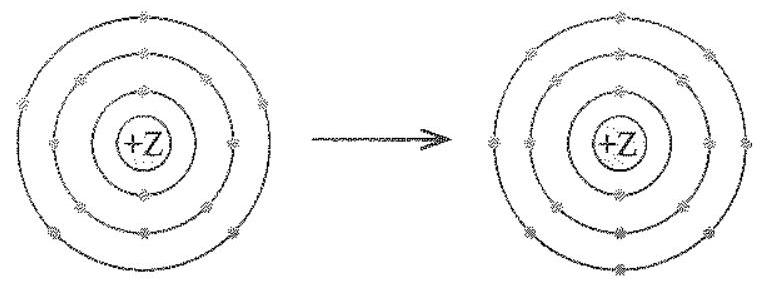
\includegraphics[max width=\textwidth, center]{2025_10_23_76620c17ffac1ae9b35bg-25(1)}\\
9.8. Nguyên tử có mô hình cấu tạo sau đây có xu hướng nhường hoặc nhận electron như thế nào khi hình thành liên kết hoá học?\\
A. Nhận 1 electron.\\
B. Nhường 1 electron.\\
C. Nhận 7 electron.\\
D. Không có xu hướng nhường hoặc nhận electron.\\
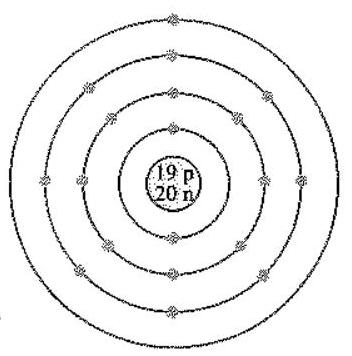
\includegraphics[max width=\textwidth, center]{2025_10_23_76620c17ffac1ae9b35bg-25}\\
9.9. Nguyên tử có mô hình cấu tạo sau sẽ có xu hướng tạo thành ion mang điện tích nào khi nó thoả mãn quy tắc octet?\\
A. $3+$.\\
B. $5+$.\\
C. 3-.\\
D. $5-$.\\
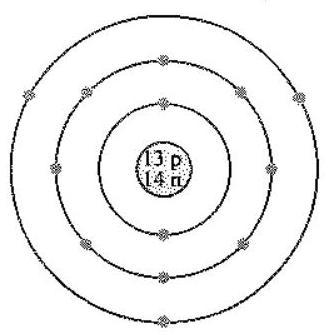
\includegraphics[max width=\textwidth, center]{2025_10_23_76620c17ffac1ae9b35bg-25(2)}\\
9.10. Em hãy vẽ mô hình mô tả quá trình tạo lớp vỏ thoả mãn quy tắc octet trong các trường hợp sau đây:\\
a) Nguyên tử $\mathrm{O}(\mathrm{Z}=8)$ nhận 2 electron để tạo anion $\mathrm{O}^{2-}$.\\
b) Nguyên tử $\mathrm{Ca}(\mathrm{Z}=20)$ nhường 2 electron để tạo cation $\mathrm{Ca}^{2+}$.\\
c) Hai nguyên tử fluorine "góp chung electron" để đạt được lớp vỏ thoả mãn quy tắc octet.
\end{enumerate}

\section*{Bal \\
 10. LIÊN KÉT ION}
10.1. Phân loại các hợp chất ion dưới đây vào các nhóm sau: hợp chất tạo nên bởi các ion đơn nguyên tử, hợp chất tạo nên bởi ion đơn nguyên tử và đa nguyên tử, hợp chất tạo nên bởi các ion đa nguyên tử.\\
$\mathrm{KCl}, \mathrm{Na}_{2} \mathrm{CO}_{3},\left(\mathrm{NH}_{4}\right)_{2} \mathrm{SO}_{4}, \mathrm{BaCO}_{3}, \mathrm{AgCl}, \mathrm{BaSO}_{4}, \mathrm{KMnO}_{4}$.\\
10.2. Cho các ion: $\mathrm{Na}^{+}, \mathrm{Ca}^{2+}, \mathrm{F}^{-}, \mathrm{CO}_{3}^{2-}$. Số lượng các hợp chất chưa hai loại ion có thể tạo thành từ các ion này là\\
A. 2 .\\
B. 3 .\\
C. 4 .\\
D. vô số hợp chất.\\
10.3. Cặp nguyên tố nào sau đây có khả năng tạo thành liên kết ion trong hợp chất của chúng?\\
A. Nitrogen và oxygen.\\
B. Carbon và hydrogen.\\
C. Sulfur và oxygen.\\
D. Calcium và oxygen.\\
10.4. Những đặc điểm nào sau đây là đúng khi nói về hợp chất tạo thành giữa $\mathrm{Na}^{+}$và $\mathrm{O}^{2-}$ ?\\
A. Là hợp chất ion.\\
B. Có công thức hoá học là NaO .\\
C. Trong điều kiện thường, tồn tại ở thể khí.\\
D. Trong điều kiện thường, tồn tại ở thể rắn.\\
E. Có nhiệt độ nóng chảy và nhiệt độ sôi cao.\\
G. Có nhiệt độ nóng chảy và nhiệt độ sôi thấp.\\
H. Lực tương tác giữa $\mathrm{Na}^{+}$và $\mathrm{O}^{2-}$ là lực tĩnh điện.\\
10.5. ZnO là một hợp chất ion được sử dụng nhiều trong kem chống nắng. Bán kính của nguyên tử O như thế nào so với bán kính của anion $\mathrm{O}^{2-}$ trong tinh thể ZnO ?\\
A. Bằng nhau.\\
B. Bán kính của O lớn hơn của $\mathrm{O}^{2-}$.

C . Bán kính của O nhỏ hơn của $\mathrm{O}^{2-}$.\\
D. Không dự đoán được.\\
10.6. Bán kính của nguyên tử Al như thế nào so với bán kính của cation $\mathrm{Al}^{3+}$ trong tinh thể $\mathrm{AlCl}_{3}$ ?\\
A. Bằng nhau.\\
B. Bán kính của Al lớn hơn của $\mathrm{Al}^{3+}$.\\
C. Bán kính của Al nhỏ hơn của $\mathrm{Al}^{3+}$.\\
D. Không đự đoán được.\\
10.7. Ghép mỗi nguyên tử ở cột A với các giá trị điện tích của ion mà nguyên tử có thể tạo thành ở cột B.

\section*{Côt A}
a) S\\
b) Al\\
c) F\\
d) Mg

\section*{Cột B}
\begin{enumerate}
  \item điện tích $2+$
  \item điện tích 3+
  \item điện tích 2-
  \item điện tích 1-\\
10.8. Chọn phương án đúng để hoàn thành câu sau:
\end{enumerate}

Khi hình thành các hợp chất ion, ...(1)... mất các electron hoá trị của chúng để tạo thành ...(2)... mang điện tích dương và ...(3)... nhận các electron hoá trị để tạo thành ...(4)... mang điện tích âm.\\
A. (1) kim loại, (2) anion, (3) phi kim, (4) cation.\\
B. (1) phi kim, (2) cation, (3) kim loại, (4) anion.\\
C. (1) kim loại, (2) ion đa nguyên tử, (3) phi kim, (4) anion.\\
D. (1) phi kim, (2) anion, (3) kim loại, (4) cation.\\
E. (1) kim loại, (2) cation, (3) phi kim, (4) anion.\\
10.9. Điền từ thích hợp vào chỗ trống:

Barium thuộc nhóm IIA, iodine thuộc nhóm VIIA, hợp chất của hai nguyên tố này là hợp chất ...(1)... Ở điều kiện thường, hợp chất này tồn tại ở thể ...(2)... với cấu trúc tinh thể tạo nên bởi ...(3)... và ...(4)...\\
10.10. Viết hai giai đoạn của sự hình thành $\mathrm{CaF}_{2}$ từ các nguyên tử tương ứng (kèm theo cấu hình electron).\\
10.11. Cho biết sự tạo thành $\mathrm{NaCl}(s)$ từ $\mathrm{Na}(s)$ và $\mathrm{Cl}_{2}(g)$ giải phóng nhiều năng lượng. Hãy cho biết năng lượng giải phóng có nguồn gốc từ đâu.\\
Gợi ý: Nếu các tiểu phân hút nhau sẽ giải phóng năng lượng, đẩy nhau sẽ hấp thu năng lượng.\\
10.12. Biết rằng năng lượng toả ra khi hình thành các hợp chất ion từ các cation và anion tỉ lệ thuận với điện tích của mỗi ion và tỉ lệ nghịch với bán kính của chúng. Dựa trên cơ sở này, hãy cho biết khi hình thành hợp chất nào trong mỗi cặp chất sau đây từ các ion tương ứng thì năng lượng toả ra là nhiều hơn.\\
a) LiCl và NaCl .\\
b) $\mathrm{Na}_{2} \mathrm{O}$ và MgO .

\section*{BAI LIÊN KẾT CỘNG HOÁ TRI}
11.1. Trong nguyên tử C , những electron có khả năng tham gia hình thành liên kết cộng hoá trị thuộc phân lớp nào sau đây?\\
A. 1 s .\\
B. 2 s .\\
C. $2 \mathrm{~s}, 2 \mathrm{p}$.\\
D. $1 \mathrm{~s}, 2 \mathrm{~s}, 2 \mathrm{p}$.\\
11.2. Những phát biểu nào sau đây là không đúng?\\
A. Các nguyên tử liên kết với nhau theo xu hướng tạo hệ bền vững hơn.\\
B. Các nguyên tử liên kết với nhau theo xu hướng tạo hệ có năng lượng thấp hơn.\\
C. Các nguyên tử liên kết với nhau theo xu hướng tạo lớp vỏ electron được octet.\\
D. Các nguyên tử liên kết với nhau theo xu hướng tạo hệ có năng lượng cao hơn.\\
E. Các nguyên tử nguyên tố phi kim chỉ liên kết với các nguyên tử nguyên tố kim loại.\\
11.3. Liên kết cộng hoá trị thường được hình thành giữa\\
A. các nguyên tử nguyên tố kim loại với nhau.\\
B. các nguyên tử nguyên tố phi kim với nhau.\\
C. các nguyên tử nguyên tố kim loại với các nguyên tử nguyên tố phi kim.\\
D. các nguyên tử khí hiếm với nhau.\\
11.4. Số lượng cặp electron dùng chung trong các phân tử $\mathrm{H}_{2}, \mathrm{O}_{2}, \mathrm{~N}_{2}, \mathrm{~F}_{2}$ lần lượt là:\\
A. $1,2,3,4$.\\
B. $1,2,3,1$.\\
C. $2,2,2,2$.\\
D. $1,2,2,1$.\\
11.5. Trong phân tử HF , số cặp electron dùng chung và cặp electron hoá trị riêng của nguyên tử F lần lượt là:\\
A. 1 và 3 .\\
B. 2 và 2 .\\
C. 3 và 1 .\\
D. 1 và 4 .\\
11.6. Cho công thức Lewis của các phân tử sau:\\
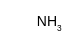
\includegraphics{smile-323b34a12f0c69f2883133db7029f44d8a3f4991}\\
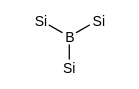
\includegraphics{smile-05655845563762e28f678febc1bb282277f475c1}

$\mathrm{H}-\mathrm{Be}-\mathrm{H}$\\
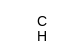
\includegraphics{smile-30674b879568ebbd9c22a96bf4ccff86b12d0434}

Số phân tử mà nguyên tử trung tâm không thoả mãn quy tắc octet là\\
A. 1 .\\
B. 2 .\\
C. 3 .\\
D. 4 .\\
11.7. Công thức nào sau đây ứng với công thức Lewis của phân tử $\mathrm{PCl}_{3}$ ?\\
A. Công thức (1).\\
B. Công thức (2).\\
C. Công thức (3).\\
D. Công thức (4).\\
E. Công thức (2) và (4).\\
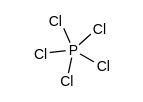
\includegraphics{smile-9415d39ed58d7d536ffe4133bc88dca68e5e4c56}

(1)\\
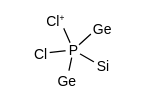
\includegraphics{smile-99b0fb6d6b6e03c90477015cbfd9ffd12b1d4fbc}

(2)\\
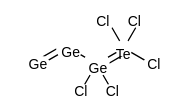
\includegraphics{smile-1aa8e2883a8d266f7ab6ad03cb0f3e1d37b64563}

(3)\\
11.8. Dựa vào hiệu độ âm điện giữa hai nguyên tố, cho biết liên kết trong phân tử nào sau đây là phân cực nhất.\\
A. HF .\\
B. HCl .\\
C. HBr .\\
D. HI.\\
11.9. Hãy điền từ/ công thức thích hợp vào chỗ trống trong đoạn thông tin sau: Trong số các hợp chất: $\mathrm{Cl}_{2}, \mathrm{H}_{2} \mathrm{O}, \mathrm{O}_{2}, \mathrm{CsF}, \mathrm{NaF}, \mathrm{SO}_{2}$, có $\ldots$ (1) $\ldots$ chất ion và ...(2)... chất cộng hoá trị. Trong điểu kiện thường, ... (3)... hợp chất tồn tại ở thể rắn là ...(4)... và ...(5)...; ...(6)... hợp chất tồn tại ở thể lỏng là ...(7)..., còn lại là các chất khí. Chất có nhiệt độ sôi, nhiệt độ nóng chảy cao nhất là ...(8) ... Trong số các chất cộng hoá trị, ...(9)..., ...(10)... là các chất cộng hoá trị phân cực; ...(11) ... và ...(12) ... là các chất cộng hoá trị không phân cực.\\
11.10. Dựa vào hiệu độ âm điện, hãy nối các liên kết hình thành giữa các nguyên tử ở cột A với loại liên kết tương ứng ở cột B .

\section*{Cột A}
a) Sr và F\\
b) N và Cl\\
c) N và O

\section*{Cột B}
\begin{enumerate}
  \item Liên kết cộng hoá trị phân cực
  \item Liên kết cộng hoá trị không phân cực
  \item Liên kết ion\\
11.11. Khi tham gia hình thành liên kết trong các phân tử $\mathrm{HF}, \mathrm{F}_{2}$; orbital tham gia xen phủ tạo liên kết của nguyên tử $F$ thuộc về phân lớp nào, có hình dạng gì?\\
A. Phân lớp 2 s , hình cầu.\\
B. Phân lớp 2 s , hình số tám nổi.\\
C. Phân lớp 2 p , hình số tám nổi.\\
D. Phân lớp 2 p , hình cánh hoa.\\
11.12. Số orbital cua cả hai nguyên tử $N$ tham gia xen phủ tạo liên kết trong phân tử $\mathrm{N}_{2}$ là\\
A. 3 .\\
B. 4 .\\
C. 5.\\
D. 6 .\\
11.13. Liên kết trong phân tử nào dưới đây không được hình thành do sự xen phủ giữa các orbital cùng loại (ví dụ cùng là orbital s , hoặc cùng là orbital p )?\\
A. $\mathrm{Cl}_{2}$.\\
B. $\mathrm{H}_{2}$.\\
C. $\mathrm{NH}_{3}$.\\
D. $\mathrm{Br}_{2}$.\\
11.14. Phát biểu nào sau đây không đủng?\\
A. Chỉ có các AO có hình dạng giống nhau mới xen phủ với nhau để tạo liên kết.\\
B. Khi hình thành liên kết cộng hoá trị giữa hai nguyên tử, luôn có một liên kết $\sigma$.\\
C. Liên kết $\sigma$ bền vững hơn liên kết $\pi$.\\
D. Có hai kiểu xen phủ hình thành liên kết là xen phủ trục và xen phủ bên.\\
11.15. Số lượng electron tham gia hình thành liên kết đơn, đôi và ba lần lượt là:\\
A. 1,2 và 3 .\\
B. 2,4 và 6 .\\
C. 1,3 và 5 .\\
D. 2,3 và 4 .\\
11.16. Ghép mỗi nguyên tử hoặc phân tử sau với một hoặc các đặc điểm tương úng của nó: $\mathrm{N}_{2}, \mathrm{Ar}, \mathrm{CO}, \mathrm{H}_{2}$.\\
(1) Liên kết trong phân tử là liên kết cộng hoá trị không phân cực.\\
(2) Liên kết trong phân tử là liên kết cộng hoá trị phân cực.\\
(3) Các nguyên tử trong phân tử đều tuân theo quy tắc octet.\\
(4) Là khí trơ.\\
(5) Có hai cặp electron hoá trị riêng.\\
(6) Liên kết trong phân tử là liên kết đơn.\\
11.17. Xét phân tử $\mathrm{H}_{2} \mathrm{O}$, những phát biểu nào sau đây là đúng?\\
A. Liên kết $\mathrm{H}-\mathrm{O}$ là liên kết cộng hoá trị không phân cực.\\
B. Liên kết $\mathrm{H}-\mathrm{O}$ là liên kết cộng hoá trị phân cực.\\
C. Cặp electron dùng chung trong liên kết $\mathrm{H}-\mathrm{O}$ lệch về phía nguyên tử O .\\
D. Cập electron dùng chung trong liên kết $\mathrm{H}-\mathrm{O}$ lệch về phía nguyên tử H .\\
E. Cặp electron dùng chung trong liên kết $\mathrm{H}-\mathrm{O}$ phân bố đều giữa hai nguyên tử.\\
G. Nguyên tử O còn hai cặp electron hoá trị riêng.\\
11.18. Xét phân tử $\mathrm{CO}_{2}$, những phát biểu nào sau đây là không đúng?\\
A. Liên kết giữa hai nguyên tử C và O là liên kết cộng hoá trị không phân cực.\\
B. Liên kết giữa hai nguyên tử C và O là liên kết cộng hoá trị phân cực.\\
C. Phân từ $\mathrm{CO}_{2}$ có 4 electron hoá trị riêng.\\
D. Phân tử $\mathrm{CO}_{2}$ có 4 cặp electron hoá trị riêng.\\
E. Trong phân tử $\mathrm{CO}_{2}$ có 3 liên kết $\sigma$ và 1 liên kết $\pi$.\\
G. Trong phân tử $\mathrm{CO}_{2}$ có 2 liên kết $\sigma$ và 2 liên kết $\pi$.\\
H. Trong phân tử $\mathrm{CO}_{2}$ có 1 liên kết $\sigma$ và 3 liên kết $\pi$.\\
11.19. Cho biết hoá trị của một nguyên tố trong phân tử bằng tổng số liên kết $\sigma$ và $\pi$ mà nguyên tử nguyên tố đó tạo thành khi liên kết với các nguyên tử xung quanh. Hoá trị của N trong $\mathrm{NH}_{4}^{+}$là\\
A. 1 .\\
B. 2 .\\
C. 3 .\\
D. 4 .\\
11.20. Cho biết năng lượng liên kết H-I và H-Br lần lượt là $297 \mathrm{~kJ} \mathrm{~mol}^{-1}$ và $364 \mathrm{~kJ} \mathrm{~mol}^{-1}$. Những phát biểu nào sau đây là không đúng?\\
A. Khi đun nóng, HI bị phân huỷ (thành $\mathrm{H}_{2}$ và $\mathrm{I}_{2}$ ) ở nhiệt độ thấp hơn so với HBr (thành $\mathrm{H}_{2}$ và $\mathrm{Br}_{2}$ ).\\
B. Liên kết $\mathrm{H}-\mathrm{Br}$ là bền vững hơn so với liên kết $\mathrm{H}-\mathrm{I}$.\\
C. Khi đun nóng, HI bị phân huỷ (thành $\mathrm{H}_{2}$ và $\mathrm{I}_{2}$ ) ở nhiệt độ cao hơn so với HBr (thành $\mathrm{H}_{2}$ và $\mathrm{Br}_{2}$ ).\\
D. Liên kết $\mathrm{H}-\mathrm{I}$ là bền vững hơn so với liên kết $\mathrm{H}-\mathrm{Br}$.\\
11.21. Cho biết năng lượng liên kết $\mathrm{H}-\mathrm{H}$ là $436 \mathrm{~kJ} \mathrm{~mol}^{-1}$. Hãy tính năng lượng cần thiết (theo eV ) để phá vỡ liên kết trong một phân tử $\mathrm{H}_{2}$, cho biết $1 \mathrm{eV}=1,602 \times 10^{-19} \mathrm{~J}$.\\
11.22. Thiết lập công thức Lewis cho các phân tử $\mathrm{H}_{2} \mathrm{O}, \mathrm{NH}_{3}$ và $\mathrm{CH}_{4}$. Mỗi phân tử này có bao nhiêu cặp electron hoá trị riêng?\\
11.23. Sử dụng bảng năng lượng của một số liên kết ở điều kiện chuẩn (Phụ lục 2, SGK Hoá học 10, Cánh Diều):\\
a) Tính tổng năng lượng liên kết trong mỗi phân tử $\mathrm{H}_{2} \mathrm{~S}$ và $\mathrm{H}_{2} \mathrm{O}$.\\
b) Nhiệt độ bắt đầu phân huỷ thành nguyên tử hai chất trên là $400^{\circ} \mathrm{C}$ và $1000^{\circ} \mathrm{C}$. Theo em, nhiệt độ phân huỷ của chất nào cao hơn? Vì sao?\\
11.24. Các phân tử như $\mathrm{F}_{2}, \mathrm{~N}_{2}$ khi phản ứng với $\mathrm{H}_{2}$ thì cần phải cắt đứt liên kết giữa các nguyển tử. Dựa vào năng lượng liên kêt, dự đoán phản ứng của $F_{2}$ hay cua $\mathrm{N}_{2}$ với $\mathrm{H}_{2}$ sẽ thuận lợi hơn (dễ xảy ra hơn). Bỏ qua ảnh hưởng của độ bền phân tử sản phẩm tới mức độ phản ứng.\\
11.25. Giải thích vì sao ở điều kiện thường không tồn tại phân tử NaCl riêng biệt mà là tinh thể NaCl .\\
12.1. Phát biểu nào sau đây là đúng?\\
A. Bất kì phân tữ nào có chứa nguyên tử hydrogen cũng có thể tạo liên kết hydrogen với phân tữ cùng loại.\\
B. Liên kết hydrogen là liên kết hình thành do sự góp chung cặp electron hoá trị giữa nguyên tử hydrogen và nguyên tử có độ âm điện lớn.\\
C. Liên kết hydrogen là loại liên kết yếu nhất giữa các phân tử.\\
D. Ảnh hưởng của liên kết hydrogen tới nhiệt độ sôi và nhiệt độ nóng chảy của chất là mạnh hơn ảnh hưởng của tương tác van der Waals.\\
12.2. Cho các phân tử: $\mathrm{H}_{2} \mathrm{O}, \mathrm{NH}_{3}, \mathrm{HF}, \mathrm{H}_{2} \mathrm{~S}, \mathrm{CO}_{2}, \mathrm{HCl}$. Số phân tử có thể tạo liên kết hydrogen với phân tử cùng loại là\\
A. 3 .\\
B. 4 .\\
C. 5.\\
D. 6 .\\
12.3. Thứ tự nào sau đây thể hiện độ mạnh giảm dần của các loại liên kết?\\
A. Liên kết ion > liên kết cộng hoá trị > liên kết hydrogen > tương tác van der Waals.\\
B. Liên kết ion > liên kết cộng hoá trị > tương tác van der Waals > liên kết hydrogen.\\
C. Liên kết cộng hoá trị > liên kết ion > liên kết hydrogen > tương tác van der Waals.\\
D. Tương tác van der Waals > liên kết hydrogen > liên kết cộng hoá trị > liên kết ion.\\
12.4. Giữa các nguyên tử He có thể có loại liên kết nào?\\
A. Liên kết cộng hoá trị.\\
B. Liên kết hydrogen.\\
C. Tương tác van der Waals.\\
D. Không có bất kì liên kết nào.\\
12.5. Quy tắc octet không được sử dụng khi xem xét sự hình thành của hai loại liên kết hoặc tương tác nào sau đây?\\
(1) Liên kết cộng hoá trị.\\
(2) Liên kết ion.\\
(3) Liên kết hydrogen.\\
(4) Tương tác van der Waals.\\
A. (1) và (2).\\
B. (2) và (3).\\
C. (1) và (3).\\
D. (3) và (4).\\
12.6. Nếu giữa phân tử chất tan và dung môi có thể tạo thành liên kết hydrogen hoặc có tương tác van der Waals càng mạnh với nhau thì càng tan tốt vào nhau.
\end{enumerate}

Lí do nào sau đây là phù hợp để giải thích dầu hoả (thành phần chính là hydrocarbon) không tan trong nước?\\
A. Cả nước và dầu đều là các phân tử có cực.\\
B. Nước là phân tử phân cực và dầu là không/ ít phân cực.\\
C. Nước là phân tử không phân cực và dầu là phân cực.\\
D. Cả nước và dầu đều không phân cực.\\
12.7. Ethanol tan vô hạn trong nước do\\
A. cả nước và ethanol đều là phân tử phân cực.\\
B. nước và ethanol có thể tạo liên kết hydrogen với nhau.\\
C. ethanol có thể tạo liên kết hydrogen với các phân tử ethanol khác.\\
D. ethanol và nước có tương tác van der Waals mạnh.\\
12.8. Chất nào trong số các chất sau tồn tại ở thể lỏng trong điều kiện thường?\\
A. $\mathrm{CH}_{3} \mathrm{OH}$.\\
B. $\mathrm{CF}_{4}$.\\
C. $\mathrm{SiH}_{4}$.\\
D. $\mathrm{CO}_{2}$.\\
12.9. Dựa vào liên kết giữa các phân tử, hãy cho biết halogen nào sau đây có nhiệt độ sôi cao nhất.\\
A. $F_{2}$.\\
B. $\mathrm{Cl}_{2}$.\\
C. $\mathrm{Br}_{2}$.\\
D. $I_{2} \cdot$\\
12.10. Hãy giải thích lí do khác nhau về nhiệt độ sôi của các cặp chất có cùng số electron sau đây: $\mathrm{CH}_{3}-\mathrm{CH}_{3}(184,5 \mathrm{~K})$ và $\mathrm{CH}_{3}-\mathrm{F}(194,7 \mathrm{~K})$.\\
12.11. Ở điều kiện thường, các khí hiếm tồn tại ở dạng khí đơn nguyên tử. Hãy giải thích sự biến đổi nhiệt độ sôi của các khí hiếm từ He tới Rn theo số liệu cho trong bảng sau:

\begin{center}
\begin{tabular}{|l|c|c|c|c|c|c|}
\hline
Khi hiếm & He & Ne & Ar & Kr & Xn & Rn \\
\hline
Sồ hiẹu nquyèn tur & 2 & 10 & 18 & 36 & 54 & 86 \\
\hline
Nhiêt độ sồ $\left.{ }^{\circ} \mathrm{C}\right)$ & -269 & -246 & -186 & -152 & -108 & -62 \\
\hline
\end{tabular}
\end{center}

12.12. Trong dung dịch, acetic acid có thể tồn tại dạng dimer (hai phân tử kết hợp) do sự hình thành liên kết hydrogen giữa hai phân tử. Hãy vẽ sơ đồ biểu diễn liên kết hydrogen giữa hai phân tử acetic acid hình thành dimer.\\
12.13*. Hãy giải thích sự biến đôi về nhiệt độ nóng chảy của dãy hydrogen halide sau.

\begin{center}
\begin{tabular}{|l|c|c|c|c|}
\hline
Halogen halide & HF & HCl & HBr & HI \\
\hline
Nhiêt đô nóng chay $(\mathrm{o} \mathrm{C})$ & $-83,1$ & $-114,8$ & $-88,5$ & $-50,8$ \\
\hline
\end{tabular}
\end{center}

12.14*. Nhiệt độ sôi của ba hợp chất được cho trong bảng sau:

\begin{center}
\begin{tabular}{|l|l|l|}
\hline
Hop chát & Khối lượng phân tur $\left(\mathrm{g} \mathrm{mol}^{-1}\right)$ & Nhiệt đô sôt ( C ) \\
\hline
2-hexanone & 100,16 & 128,0 \\
\hline
heptane & 100,20 & 98,0 \\
\hline
1-hexanol & 102,17 & 156,0 \\
\hline
\end{tabular}
\end{center}

Không cần tra cứu cấu trúc, em hãy trả lời các câu hỏi sau về ba hợp chất này:\\
a) Hợp chất nào có thể hình thành liên kết hydrogen?\\
b) Hợp chất nào phân cực nhưng không hình thành liên kết hydrogen?\\
c) Hợp chất nào ít phân cực, không tạo liên kết hydrogen?

\section*{CHỦ DỀ 4: PHẢN ỨNG OXI HOÁ - KHỬ}
\section*{Bat 13 PHẢN ÚNG OXI HOÁ - KHỦ}
13.1. Phát biểu nào sau đây là đúng?\\
A. Số oxi hoá của nguyên tử trong bất kì một đơn chất hoá học nào đều bằng 0 .\\
B. Tổng số oxi hoá của tất cả các nguyên tử trong một phân tử và trong một ion đa nguyên tử bằng 0 .\\
C. Trong tất cả các hợp chất, hydrogen luôn có số oxi hoá là +1 .\\
D. Trong tất cả các hợp chất, oxygen luôn có số oxi hoá là -2 .\\
13.2. Phát biểu nào sau đây không đúng?\\
A. Số oxi hoá của một nguyên tử một nguyên tố trong hợp chất là điện tích của nguyên tử đó với giả thiết đó là hợp chất ion.\\
B. Trong hợp chất, oxygen có số oxi hoá bằng -2 , trừ một số trường hợp ngoại lệ.\\
C. Số oxi hoá của hydrogen trong các hydride kim loại bằng +1 .\\
D. Các nguyên tố phi kim có số oxi hoá thay đổi tuỳ thuộc vào hợp chất chứa chúng.\\
13.3. Số oxi hoá của chromium ( Cr ) trong $\mathrm{Na}_{2} \mathrm{CrO}_{4}$ là\\
A. -2 .\\
B. +2 .\\
C. +6 .\\
D. -6 .\\
13.4. Số oxi hoá của carbon và oxygen trong $\mathrm{C}_{2} \mathrm{O}_{4}^{2-}$ lần lượt là:\\
A. $+3,-2$.\\
B. $+4,-2$.\\
C. $+1,-3$.\\
D. $+3,-6$.\\
13.5. Số oxi hoá của Cl trong các chất $\mathrm{NaOCl}, \mathrm{NaClO}_{2}, \mathrm{NaClO}_{3}, \mathrm{NaClO}_{4}$ lần lượt là:\\
A. $-1,+3,+5,+7$.\\
B. $+1,-3,+5,-2$.\\
C. $+1,+3,+5,+7$.\\
D. $+1,+3,-5,+7$.\\
13.6. a) Xác định số oxi hoá của mỗi nguyên tử trong các chất hoá học hoặc các ion sau: $\mathrm{NO}_{3}^{-} ; \mathrm{H}_{2} \mathrm{PO}_{4}^{-} ; \mathrm{CaHAsO}_{4} ; \mathrm{Mg}_{2} \mathrm{TiO}_{4}$.\\
b) Ghép phân tữ/ ion ở cột A với nhóm số oxi hoá của các nguyên tử trong phân tữ/ ion ở cột B cho phù hợp.

Côt A\\
Phân tữ/ ion\\
a) $\mathrm{SbCl}_{5}$\\
b) $\mathrm{BrO}_{3}^{-}$\\
c) $\mathrm{Na}_{2} \mathrm{O}_{2}$\\
d) $\mathrm{Na}_{2} \mathrm{~S}$\\
e) $\mathrm{NH}_{4}^{+}$

Côt B\\
Số oxi hoá của các nguyên tử trong phân tữ/ ion (lần lượt theo thứ tự như trong phân tư/ ion)

\begin{enumerate}
  \item $(-3 ;+1)$
  \item $(+5 ;-1)$
  \item $(+1 ;-2)$
  \item $(+1 ;-1)$
  \item $(+5 ;-2)$
  \item $(-1 ;+2)$\\
13.7. Dựa vào công thức cấu tạo, hãy xác định số oxi hoá của mỗi nguyên tố trong các hợp chất sau.
\end{enumerate}

\begin{center}
\begin{tabular}{|l|l|l|l|}
\hline
Phân tư/ Ion & Công thưre cáu tạo & Phân tư/ Ion & Công thức cáu tạo \\
\hline
$\mathrm{CaCO}_{3}$ & \( [\mathrm{Ca}]^{2+}\left[\begin{array}{rrr} \mathrm{O} & \\ & \mathrm{II} & \\ & \mathrm{C} & \\ -\mathrm{O}^{-} & & \mathrm{O}^{-} \end{array}\right]^{2-} \) & $\mathrm{H}_{2} \mathrm{SO}_{4}$ & 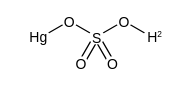
\includegraphics{smile-8ef5e0b828b9759ef1122581d449fec086bc6763} \\
\hline
$\mathrm{NH}_{4}^{+}$ & 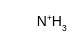
\includegraphics{smile-2c1078cf70db4d457597b44a22a272e894267bb7} & $\mathrm{CaH}_{2}$ & $\mathrm{H}-\mathrm{Ca}-\mathrm{H}$ \\
\hline
\end{tabular}
\end{center}

13.8*. Magnetite là một loại sắt oxide có công thức $\mathrm{Fe}_{3} \mathrm{O}_{4}$ (còn gọi là oxit sắt từ). Chất này được coi là hỗn hợp của hai oxide. Tìm hiểu và xác định số oxi hoá của từng nguyên tử Fe trong magnetite.\\
13.9. Những phát biểu nào sau đây đúng?\\
A. Sự oxi hoá là sự nhường electron hay sự làm tăng số oxi hoá.\\
B. Trong quá trình oxi hoá, chất khử nhận electron.\\
C. Sự khử là sự nhận electron hay là sự làm giảm số oxi hoá.\\
D. Trong quá trình khử, chất oxi hoá nhường electron.\\
E. Trong quá trình khử, chất oxi hoá nhận electron và bị khử xuống số oxi hoá thấp hơn.\\
G. Trong quá trình oxi hoá, chất khử nhường electron và bị oxi hoá lên số oxi hoá cao hon.\\
13.10. Những phát biểu nào sau đây không đúng?\\
A. Chất khử (chất bị oxi hoá) là chất nhường electron và chất oxi hoá (chất bị khừ) là chất nhận electron.\\
B. Quá trình nhường electron là quá trình khử và quá trình nhận electron là quá trình oxi hoá.\\
C. Trong quá trình oxi hoá, chất oxi hoá bị oxi hoá lên số oxi hoá cao hơn.\\
D. Trong quá trình khử, chất khử bị khử xuống số oxi hoá thấp hơn.\\
E. Phản ứng trong đó có sự trao đổi electron là phản ứng oxi hoá - khử.\\
G. Trong phản ứng oxi hoá - khử, sự oxi hoá và sự khử luôn xảy ra đồng thời.\\
13.11. Điền vào chỗ trống trong đoạn thông tin sau:

Phản ứng $\mathrm{Fe}_{2} \mathrm{O}_{3}+\mathrm{CO} \rightarrow \mathrm{Fe}+\mathrm{CO}_{2}$ xảy ra trong quá trình luyện gang từ quặng hematite là phản ứng ...(1)... vì có sự thay đổi ...(2) ... của các nguyên tố Fe và $\mathrm{C} . \mathrm{CO}$ là ...(3)..., trong đó $\stackrel{+2}{\mathrm{C}} \ldots$ (4)... electron và $\mathrm{Fe}_{2} \mathrm{O}_{3}$ là ...(5)..., trong đó mồi $\stackrel{+3}{\mathrm{Fe}}$...(6)... electron.\\
13.12. Trong công nghiệp, sulfuric acid được sản xuất từ quặng pirite sắt có thành phần chính là $\mathrm{FeS}_{2}$ theo sơ đồ sau:

$$
\mathrm{FeS}_{2} \rightarrow \mathrm{SO}_{2} \rightarrow \mathrm{SO}_{3} \rightarrow \mathrm{H}_{2} \mathrm{SO}_{4}
$$

a) Hoàn thành sơ đồ trên bằng các phương trình hoá học, cân bằng các phương trình hoá học đó. Trong sơ đồ trên, những phản ứng nào là phản ứng oxi hoá - khử? Chỉ rõ chất khử và chất oxi hoá của mỗi phản ứng đó.\\
b) Tính khối lượng $\mathrm{H}_{2} \mathrm{SO}_{4} 98 \%$ điều chế được từ 1 tấn quặng chưa $60 \% \mathrm{FeS}_{2}$. Biết hiệu suất cả quá trình là $80 \%$.\\
c) Đề xuất một công thức cấu tạo phù hợp cho $\mathrm{FeS}_{2}$, biết S có số oxi hoá -1 trong chất này.\\
13.13. Trong những phản ưng hoá học xảy ra theo các phương trình dưới đây, những phản ứng nào là phản úng oxi hoá - khử?\\
(1) $\mathrm{PCl}_{3}+\mathrm{Cl}_{2} \rightarrow \mathrm{PCl}_{5}$\\
(2) $\mathrm{Cu}+2 \mathrm{AgNO}_{3} \rightarrow \mathrm{Cu}\left(\mathrm{NO}_{3}\right)_{2}+2 \mathrm{Ag}$\\
(3) $\mathrm{CO}_{2}+2 \mathrm{LiOH} \rightarrow \mathrm{Li}_{2} \mathrm{CO}_{3}+\mathrm{H}_{2} \mathrm{O}$\\
(4) $\mathrm{FeCl}_{2}+2 \mathrm{NaOH} \rightarrow \mathrm{Fe}(\mathrm{OH})_{2}+2 \mathrm{NaCl}$

Chọn phương án đúng.\\
A. (3).\\
B. (4).\\
C. (1) và (2).\\
D. (1), (2) và (3).

Với phương án đã chọn, chỉ ra chất khử, chất oxi hoá và viết các quá trình oxi hoá và quá trình khử tương úng,\\
13.14. Hãy xác định chất bị khử, chất bị oxi hoá trong các phản ứng hoá học dưới đây.\\
a) $2 \mathrm{HNO}_{3}+3 \mathrm{H}_{3} \mathrm{AsO}_{3} \rightarrow 2 \mathrm{NO}+3 \mathrm{H}_{3} \mathrm{AsO}_{4}+\mathrm{H}_{2} \mathrm{O}$\\
b) $\mathrm{NaI}+3 \mathrm{HOCl} \rightarrow \mathrm{NaIO}_{3}+3 \mathrm{HCl}$\\
c) $2 \mathrm{KMnO}_{4}+5 \mathrm{H}_{2} \mathrm{C}_{2} \mathrm{O}_{4}+3 \mathrm{H}_{2} \mathrm{SO}_{4} \rightarrow 10 \mathrm{CO}_{2}+\mathrm{K}_{2} \mathrm{SO}_{4}+2 \mathrm{MnSO}_{4}+8 \mathrm{H}_{2} \mathrm{O}$\\
d) $6 \mathrm{H}_{2} \mathrm{SO}_{4}+2 \mathrm{Al} \rightarrow \mathrm{Al}_{2}\left(\mathrm{SO}_{4}\right)_{3}+3 \mathrm{SO}_{2}+6 \mathrm{H}_{2} \mathrm{O}$\\
13.15. Viết các phản ứng cho quá trình oxi hoá, quá trình khử và cân bằng các phản ứng sau:\\
a) $\mathrm{Ag}+\mathrm{Fe}^{2+} \rightarrow \mathrm{Ag}^{+}+\mathrm{Fe}$\\
b) $\mathrm{Cr}^{3+}+\mathrm{Zn} \rightarrow \mathrm{Cr}+\mathrm{Zn}^{2+}$\\
c) $\mathrm{CH}_{4}+\mathrm{O}_{2} \rightarrow \mathrm{CO}_{2}+\mathrm{H}_{2} \mathrm{O}$\\
d) $\mathrm{MnO}_{2}+\mathrm{Al} \rightarrow \mathrm{Mn}+\mathrm{Al}_{2} \mathrm{O}_{3}$\\
13.16. Một số loại xe ô tô được trang bị một thiết bị an toàn là túi chứa một lượng nhất định hợp chất ion sodium azide ( $\mathrm{NaN}_{3}$ ), được gọi là "túi khi". Khi có va chạm mạnh xảy ra, sodium azide bị phân huỷ rất nhanh, giải phóng khí $\mathrm{N}_{2}$ và nguyên tố Na, làm túi phồng lên, bảo vệ được người trong xe tránh khỏi thương tích. Viết phương trình hoá học của phản ứng xảy ra và xác định đây có phải là phản ứng oxi hoá - khử không. Vì sao? Xác định số oxi hoá của mỗi nguyên tử trong $\mathrm{NaN}_{3}$.\\
13.17*. Sự cháy của hydrocarbon trong oxygen:

Quá trình đốt cháy nhiên liệu (khí đốt, xăng, dầu hoặc khí hoá lỏng) là một ví dụ về sự cháy của hydrocarbon trong oxygen và cung cấp cho chúng ta năng lượng. Nếu oxygen dư thì sự cháy xảy ra hoàn toàn và cho sản phẩm là $\mathrm{CO}_{2}$ và nước. Nếu thiếu oxygen, sự cháy xảy ra không hoàn toàn và một phần carbon chuyển thành CO là một khí độc, gây ô nhiễm môi trường. Còn khi rất thiếu oxygen thì chỉ tạo ra nước và để lại muội là carbon. Hãy viết các phương trình hoá học cho phản ứng cháy của xăng (octane $-\mathrm{C}_{8} \mathrm{H}_{18}$ ) trong ba điều kiện: dư oxygen, không dư oxygen và rất thiếu oxygen. Theo em, điều kiện nào sẽ tiết kiệm năng lượng nhất? Vì sao? Trong điều kiện đó, một phân tử $\mathrm{C}_{8} \mathrm{H}_{18}$ sẽ nhường bao nhiêu electron?

\section*{CHỦ ĐỀ 5: NĂNG LƯỢNG HOÁ HOC}
\section*{Bet}
\begin{enumerate}
  \setcounter{enumi}{13}
  \item PHẢN ÚNG HOÁ HOC VÀ ENTHALPY\\
14.1. Những phát biểu nào sau đây là đúng?\\
A. Tất cả các phản ứng cháy đều toả nhiệt.\\
B. Phản ứng toả nhiệt là phản ứng giải phóng năng lượng dưới dạng nhiệt.\\
C. Tất cả các phản ứng mà chất tham gia có chứa nguyên tố oxygen đều toả nhiệt.\\
D. Phản ứng thu nhiệt là phản ứng hấp thụ năng lượng dưới dạng nhiệt.\\
E. Lượng nhiệt mà phản ứng hấp thụ hay giải phóng không phụ thuộc vào điều kiện thực hiện phản ứng và thể tồn tại của chất trong phản ứng.\\
G. Sự cháy của nhiên liệu (xăng, dầu, khí gas, than, gỗ,...) là những ví dụ về phản ứng thu nhiệt vì cần phải khơi mào.\\
14.2. Những phát biểu nào sau đây là không đúng?\\
A. Trong phòng thí nghiệm, có thể nhận biết một phản ứng thu nhiệt hoặc toả nhiệt bằng cách đo nhiệt độ của phản ứng bằng một nhiệt kế.\\
B. Nhiệt độ của hệ phản ứng sẽ tăng lên nếu phản ứng thu nhiệt.\\
C. Nhiệt độ của hệ phản ứng sẽ tăng lên nếu phản ứng toả nhiệt.\\
D. Nhiệt độ của hệ phản ứng sẽ giảm đi nếu phản ứng toả nhiệt.\\
E. Nhiệt độ của hệ phản ứng sẽ giảm đi nếu phản ứng thu nhiệt.\\
14.3. Phát biểu nào sau đây đúng?\\
A. Điều kiện chuẩn là điều kiện ứng với áp suất 1 bar (với chất khí), nồng độ $1 \mathrm{~mol} \mathrm{~L}^{-1}$ (đối với chất tan trong dung dịch) và nhiệt độ thường được chọn là 298 K .\\
B. Điều kiện chuẩn là điều kiện ứng với nhiệt độ 298 K .\\
C. Áp suất 760 mmHg là áp suất ở điều kiện chuẩn.\\
D. Điều kiện chuẩn là điều kiện ứng với áp suất 1 atm , nhiệt độ $0^{\circ} \mathrm{C}$.\\
14.4. Mỗi quá trình sau đây là thu nhiệt hay toả nhiệt?\\
(1) $\mathrm{H}_{2} \mathrm{O}$ (lóng, ở $\left.25^{\circ} \mathrm{C}\right) \rightarrow \mathrm{H}_{2} \mathrm{O}$ (hơi, ở $100^{\circ} \mathrm{C}$ ).\\
(2) $\mathrm{H}_{2} \mathrm{O}$ (lỏng, ở $\left.25^{\circ} \mathrm{C}\right) \rightarrow \mathrm{H}_{2} \mathrm{O}$ (rắn, ở $0^{\circ} \mathrm{C}$ ).\\
(3) $\mathrm{CaCO}_{3}$ (Đá vôi) $\xrightarrow{\text { Nung }} \mathrm{CaO}+\mathrm{CO}_{2}$.\\
(4) Khí methane $\left(\mathrm{CH}_{4}\right)$ cháy trong oxygen.\\
14.5. Biết rằng ở điều kiện chuẩn, 1 mol ethanol cháy toả ra một lượng nhiệt là $1,37 \times 10^{3} \mathrm{~kJ}$. Nếu đốt cháy hoàn toàn 15,1 gam ethanol, năng lượng được giải phóng ra dưới dạng nhiệt bởi phản ứng là\\
A. $0,450 \mathrm{~kJ}$.\\
B. $2,25 \times 10^{3} \mathrm{~kJ}$.\\
C. $4,50 \times 10^{2} \mathrm{~kJ}$.\\
D. $1,37 \times 10^{3} \mathrm{~kJ}$.\\
14.6. Chọn câu trả lời đúng.
\end{enumerate}

Enthalpy tạo thành chuẩn của một đơn chất bền\\
A. là biến thiên enthalpy chuẩn của phản ứng giữa nguyên tố đó với hydrogen.\\
B. là biến thiên enthalpy chuẩn của phản ứng giữa nguyên tố đó với oxygen.\\
C. được xác định từ nhiệt độ nóng chảy của nguyên tố đó.\\
D. bằng 0 .\\
14.7. Những phát biểu nào sau đây đúng?\\
A. Biến thiên enthalpy chuẩn của một phản ứng hoá học là lượng nhiệt kèm theo phản ứng đó ở áp suất 1 atm và $25^{\circ} \mathrm{C}$.\\
B. Nhiệt (toả ra hay thu vào) kèm theo một phản ứng được thực hiện ở 1 bar và 298 K là biến thiên enthalpy chuẩn của phản ưng đó.\\
C. Một số phản ứng khi xảy ra làm môi trương xung quanh nóng lên là phản ứng thu nhiệt.\\
D. Một số phản ứng khi xảy ra làm môi trường xung quanh lạnh đi là do các phản ứng này thu nhiệt và lấy nhiệt từ môi trường.\\
14.8. Cho hai phản ứng cùng xảy ra ở điều kiện chuẩn:\\
(1) $\mathrm{N}_{2}(g)+\mathrm{O}_{2}(g) \rightarrow 2 \mathrm{NO}(g) \Delta_{\mathrm{r}} \mathrm{H}_{298(1)}^{0}$\\
(2) $\mathrm{NO}(g)+\frac{1}{2} \mathrm{O}_{2}(g) \rightarrow \mathrm{NO}_{2}(g) \Delta_{\mathrm{r}} \mathrm{H}_{298(2)}^{0}$

Những phát biểu nào sau đây không đúng?\\
A. Enthalpy tạo thành chuẩn của NO là $\frac{1}{2} \Delta_{\mathrm{r}} \mathrm{H}_{298(1)}^{0} \mathrm{~kJ} \mathrm{~mol}^{-1}$.\\
B. Enthalpy tạo thành chuẩn của $\mathrm{NO}_{2}$ là $\Delta_{\mathrm{r}} \mathrm{H}_{298(2)}^{0} \mathrm{~kJ} \mathrm{~mol}^{-1}$.\\
C. Biến thiên enthalpy chuẩn của phản ứng giữa $1 \mathrm{~mol} \mathrm{~N}_{2}$ với $1 \mathrm{~mol} \mathrm{O}_{2}$ tạo thành 2 mol NO là $\frac{1}{2} \Delta_{\mathrm{r}} \mathrm{H}_{298(1)}^{0} \mathrm{~kJ}$.\\
D. Biến thiên enthalpy chuẩn của phản ứng giữa 1 mol khí NO với $0,5 \mathrm{~mol}$ khí $\mathrm{O}_{2}$ tạo thành 1 mol khí $\mathrm{NO}_{2}$ là $\triangle_{\mathrm{r}} \mathrm{H}_{298(2)}^{0} \mathrm{~kJ}$.\\
E. Enthalpy tạo thành chuẩn của $\mathrm{NO}_{2}(g)$ là:

$$
\frac{1}{2} \Delta_{\mathrm{r}} \mathrm{H}_{298(1)}^{0}+\Delta_{\mathrm{r}} \mathrm{H}_{298(2)}^{0}\left(\mathrm{~kJ} \mathrm{~mol}^{-1}\right) .
$$

14.9. Phản ứng phân huỷ $1 \mathrm{~mol} \mathrm{H}_{2} \mathrm{O}(g)$ ở điều kiện chuẩn:


\begin{equation*}
\mathrm{H}_{2} \mathrm{O}(g) \rightarrow \mathrm{H}_{2}(g)+\frac{1}{2} \mathrm{O}_{2}(g) \tag{1}
\end{equation*}


cần cung cấp một nhiệt lượng là $241,8 \mathrm{~kJ}$.\\
Điền vào chỗ trống trong các phát biểu dưới đây:\\
a) Phản ứng (1) là phản ứng $\_\_\_\_$ nhiệt.\\
b) Nhiệt tạo thành chuẩn của $\mathrm{H}_{2} \mathrm{O}(g)$ là $\_\_\_\_$\\
c) Biến thiên enthalpy chuẩn của phản ứng $2 \mathrm{H}_{2}(g)+\mathrm{O}_{2}(g) \rightarrow 2 \mathrm{H}_{2} \mathrm{O}(g)$ là $\_\_\_\_$\\
d) Biến thiên enthalpy chuẩn của phản ứng (1) là $\_\_\_\_$\\
14.10. Phương trình hoá học nào dưới đây biểu thị enthalpy tạo thành chuẩn của $\mathrm{CO}(g)$ ?\\
A. 2 C (than chì) $+\mathrm{O}_{2}(g) \rightarrow 2 \mathrm{CO}(g)$\\
B. C (than chì) $+\mathrm{O}(g) \rightarrow \mathrm{CO}(g)$\\
C. $\mathrm{C}($ than chi) $)+\frac{1}{2} \mathrm{O}_{2}(g) \rightarrow \mathrm{CO}(g)$\\
D. $\mathrm{C}($ than chì $)+\mathrm{CO}_{2}(g) \rightarrow 2 \mathrm{CO}(g)$\\
E. $\mathrm{CO}(g) \rightarrow \mathrm{C}($ than chì $)+\mathrm{O}(g)$\\
14.11. Khi pha loãng $100 \mathrm{~mL} \mathrm{H}_{2} \mathrm{SO}_{4}$ đặc bằng nước thấy cốc đựng dung dịch nóng lên. Vậy quá trình pha loãng $\mathrm{H}_{2} \mathrm{SO}_{4}$ đặc là quá trình thu nhiệt hay toả nhiệt? Theo em, khi pha loãng $\mathrm{H}_{2} \mathrm{SO}_{4}$ đặc nên cho từ từ $\mathrm{H}_{2} \mathrm{SO}_{4}$ đặc vào nước hay ngược lại? Ví sao?\\
14.12. Nhiệt toả ra khi đốt cháy 1 gam một mẫu than là $23,0 \mathrm{~kJ}$. Giả thiết rằng toàn bộ lượng nhiệt của quá trình đốt than toả ra đều dùng để làm nóng nước, không có sự thất thoát nhiệt, hãy tính lượng than cần phải đốt để làm nóng 500 gam nước từ $20^{\circ} \mathrm{C}$ tới $90^{\circ} \mathrm{C}$. Biết để làm nóng 1 mol nước thêm $1^{\circ} \mathrm{C}$ cần một nhiệt lượng là $75,4 \mathrm{~J}$.\\
14.13*. Ethanol sôi ở $78,29^{\circ} \mathrm{C}$. Để làm 1 gam ethanol lỏng nóng thêm $1^{\circ} \mathrm{C}$ cần một nhiệt lượng là $1,44 \mathrm{~J}$; để 1 gam ethanol hoá hơi ( $0^{3} 78,29^{\circ} \mathrm{C}$ ) cần một nhiệt lượng là 855 J . Hãy tính lượng nhiệt cần cung cấp để làm nóng 1 kg ethanol từ $20,0^{\circ} \mathrm{C}$ đến nhiệt độ sôi và hoá hơi hoàn toàn ở nhiệt độ đó.

\section*{BAI Ý NGHĨA VÀ CÁCH TÍNH BIẾN THIÊN ENTHALPY 15 PHẢN ÚNG HOÁ HOC}
15.1. Nối mỗi nội dung ở cột A với nội dung ở cột B cho phù hợp:

\section*{Cột A}
a) Trong phản ứng thu nhiệt, dấu của $\Delta \mathrm{H}$ dương vì\\
b) Trong phản ứng toả nhiệt có sự\\
c) Trong phản ứng toả nhiệt, $\Delta \mathrm{H}$ có dấu âm vì\\
d) Trong phản ứng thu nhiệt có sự

\section*{Cột B}
\begin{enumerate}
  \item giải phóng năng lượng.
  \item hấp thụ năng lượng.
  \item năng lượng của hệ chất phản ứng lớn hơn năng lượng của hệ chất sản phẩm.
  \item năng lượng của hệ chất phản ứng nhỏ hơn năng lượng của hệ chất sản phẩm.\\
15.2. Đường sucrose $\left(\mathrm{C}_{12} \mathrm{H}_{22} \mathrm{O}_{11}\right)$ là một đường đôi. Trong môi trường acid ở dạ dày và nhiệt độ cơ thể, sucrose bị thuỷ phân thành đường glucose và fructose, sau đó bị oxi hoá bởi oxygen tạo thành $\mathrm{CO}_{2}$ và $\mathrm{H}_{2} \mathrm{O}$. Sơ đồ thay đổi năng lượng hoá học của phản ứng được cho như hình dưới đây:\\
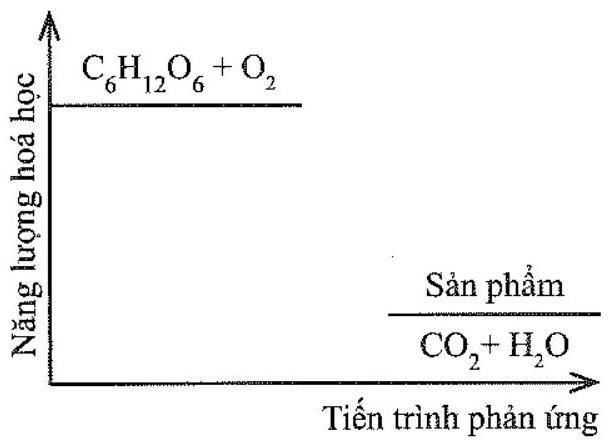
\includegraphics[max width=\textwidth, center]{2025_10_23_76620c17ffac1ae9b35bg-42}\\
a) Dựa theo đồ thị, hãy cho biết phản ứng trong đó là toả nhiệt hay thu nhiệt. Ví sao?\\
b) Viết phương trình hoá học của phản ứng thuỷ phân đường sucrose. Phản ứng trong so đồ có phải là phản ứng oxi hoá - khử không? Nếu có, hãy chỉ ra chất oxi hoá và chất khử trong phản ứng và cân bằng phương trình hoá học của phản ứng theo phương pháp thăng bằng electron.\\
c) Khi 1 mol đường sucrose bị đốt cháy hoàn toàn với một lượng vừa đủ oxygen ở điều kiện chuẩn toả ra một lượng nhiệt là 5645 kJ . Xác định biến thiên enthalpy chuẩn của phản ứng oxi hoá sucrose.\\
d) Nếu 5,00 gam đường sucrose được đốt cháy hoàn toàn ở cùng điều kiện như trên thì biến thiên enthalpy quá trình bằng bao nhiêu?\\
e) Vì sao để duy trì một cơ thể khoẻ mạnh, cần một chế độ dinh duỡng đầy đủ và luyện tập thể dục thể thao hợp lí?\\
15.3*. Biến thiên enthalpy chuẩn của quá trình " $\mathrm{H}_{2} \mathrm{O}(s) \rightarrow \mathrm{H}_{2} \mathrm{O}(l)$ " là $6,020 \mathrm{~kJ}$.\\
a) Quá trình tan chảy của nước đá là quá trình thu nhiệt hay toả nhiệt? Vì sao?\\
b) Vì sao khi cho viên nước đá vào một cốc nước lỏng ấm, viên đá lại tan chảy dần?\\
c) Vì sao cốc nước lỏng bị lạnh dần trong quá trình viên nước đá tan chảy?\\
d) Biết rằng để làm cho nhiệt độ của 1 mol nước lỏng thay đổi $1^{\circ} \mathrm{C}$ cần một nhiệt lượng là $75,4 \mathrm{~J}$. Giả sử mỗi viên nước đá tương ứng với 1 mol nước, số viên nước đá tối thiểu cần tan chảy để có thể làm lạnh 500 gam nước lỏng ở $20^{\circ} \mathrm{C}$ xuống $0^{\circ} \mathrm{C}$ là\\
A. 1 .\\
B. 7 .\\
C. 14.\\
D. 15 .\\
E. 126.\\
e) Để làm lạnh 120 gam nước lỏng ở $45^{\circ} \mathrm{C}$ xuống $0^{\circ} \mathrm{C}$, một bạn học sinh đã dùng 150 gam nước đá. Lượng nước đá này là vừa đủ, thiếu hay dư?\\
(Trong phần $\mathrm{d}, \mathrm{e}$, giả thiết chỉ có sự trao đổi nhiệt giữa nước và nước đá.)\\
15.4. Phản ứng của 1 mol ethanol lỏng với oxygen xảy ra theo phương trình:
\end{enumerate}


\begin{equation*}
\mathrm{C}_{2} \mathrm{H}_{5} \mathrm{OH}(l)+\mathrm{O}_{2}(g) \rightarrow \mathrm{CO}_{2}(g)+\mathrm{H}_{2} \mathrm{O}(l) \tag{1}
\end{equation*}


a) Những nhận định nào sau đây là đúng?\\
(1) Đây là phản ứng toả nhiệt vì nó tạo ra khí $\mathrm{CO}_{2}$ và nước lỏng.\\
(2) Đây là phải là phản ứng oxi hoá - khử với tổng số hệ số cân bằng trong phương trình phản ứng là 9 .\\
(3) Biến thiên enthalpy chuẩn của phản ứng sẽ thay đổi nếu nước được tạo ra ở thể khí.\\
(4) Sản phẩm của phản ứng chiểm một thể tích lớn hơn so với chất phản ứng.\\
A. (1), (2).\\
B. (1), (2), (3).\\
C. (1), (3), (4).\\
D. (3), (4).\\
E. (1).\\
G. (2), (3).\\
b) Biến thiên enthalpy chuẩn kèm theo quá trình khi 1 mol ethanol lỏng cháy hoàn toàn trong oxygen là $\Delta_{\mathrm{r}} \mathrm{H}_{298}^{0}=-1,367 \times 10^{3} \mathrm{~kJ}$, xác định enthalpy hình thành chuẩn của $\mathrm{C}_{2} \mathrm{H}_{5} \mathrm{OH}$ (lỏng).\\
(Những số liệu cần thiết được cho trong Phụl lục 3, SGK Hoá học 10, Cánh Diều.)\\
15.5. Sulfur dioxide là một chất có nhiều ứng dụng trong công nghiệp (dùng để sản xuất sulfuric acid, tẩy trắng bột giấy trong công nghiệp giấy, tẩy trắng dung dịch đường trong sản xuất đường tinh luyện,...) và giúp ngăn cản sự phát triển của một số loại vi khuẩn và nấm gây hư hại cho thực phẩm. Ở áp suất 1 bar và nhiệt độ $25^{\circ} \mathrm{C}$, phản ứng giữa 1 mol sulfur với oxygen xảy ra theo phương trình " $\mathrm{S}(\mathrm{s})+\mathrm{O}_{2}(\mathrm{~g}) \rightarrow \mathrm{SO}_{2}(\mathrm{~g})$ " và toả ra một lượng nhiệt là $296,9 \mathrm{~kJ}$.\\
Những phát biểu nào sau đây là đúng?\\
A. Biến thiên enthalpy chuẩn của phản ứng là $296,9 \mathrm{~kJ}$.\\
B. Enthalpy tạo thành chuẩn của sulfur dioxide bằng $-296,9 \mathrm{~kJ} \mathrm{~mol}^{-1}$.\\
C. Sulfur dioxide vừa có thể là chất khử vừa có thể là chất oxi hoá, tuỳ thuộc vào phản ứng mà nó tham gia.\\
D. $0,5 \mathrm{~mol}$ sulfur tác dụng hết với oxygen giải phóng $148,45 \mathrm{~kJ}$ năng lượng dưới dạng nhiệt.\\
E. 32 gam sulfur cháy hoàn toàn toả ra một lượng nhiệt là $2,969 \times 10^{5} \mathrm{~J}$.\\
15.6. Phản ứng luyện gang trong lò cao có phương trình như sau:


\begin{equation*}
\mathrm{Fe}_{2} \mathrm{O}_{3}(s)+\mathrm{CO}(g) \rightarrow \mathrm{Fe}(s)+\mathrm{CO}_{2}(g) \tag{1}
\end{equation*}


a) Cân bằng phương trình hoá học của phản ứng (1) và tính biến thiên enthalpy chuẩn của phản ứng với các hệ số cân bằng tương ứng.\\
b) Từ $1 \mathrm{~mol} \mathrm{Fe}_{2} \mathrm{O}_{3}$ và 1 mol CO , giả sử chỉ xảy ra phản ứng (1) với hiệu suất $100 \%$ thì giải phóng một lượng nhiệt là\\
A. $8,27 \mathrm{~kJ}$.\\
B. $49,6 \mathrm{~kJ}$.\\
C. $12,4 \mathrm{~kJ}$.\\
D. $74,4 \mathrm{~kJ}$.\\
(Các số liệu cần thiết tra trong Phụ lục 3, SGK Hoá học 10, Cánh Diều.)\\
15.7. Ở điều kiện chuẩn, 2 mol nhôm tác dụng vừa đủ với khí chlorine tạo muối aluminium chloride và giải phóng một lượng nhiệt $1390,81 \mathrm{~kJ}$.\\
a) Viết và cân bằng phương trình hoá học của phản ứng. Đây có phải phản ứng oxi hoá - khử không? Vì sao?\\
b) Biến thiên enthalpy chuẩn của phản ứng bằng bao nhiêu? Phản ứng trên thu nhiệt hay toả nhiệt?\\
c) Tính lượng nhiệt được giải phóng khi 10 gam $\mathrm{AlCl}_{3}$ được tạo thành.\\
d) Nếu muốn tạo ra được $1,0 \mathrm{~kJ}$ nhiệt lượng cần bao nhiêu gam Al phản ứng?\\
15.8. Trong ngành công nghệ lọc hoá dầu, các ankan thường được loại bỏ hydrogen trong các phản ứng dehydro hoá để tạo ra những sản phẩm hydrocarbon không no có nhiều ứng dụng trong công nghiệp. Hãy tính biến thiên enthalpy chuẩn của các phản ứng sau dựa vào năng lượng liên kết. (Giá trị một số năng lượng liên kết được cho trong Phụ lục 2, SGK Hoá học 10 , Cánh Diều)\\
a) $\mathrm{H}_{3} \mathrm{C}-\mathrm{CH}_{2}-\mathrm{CH}_{2}-\mathrm{CH}_{3} \rightarrow \mathrm{CH}_{2}=\mathrm{CH}-\mathrm{CH}=\mathrm{CH}_{2}+2 \mathrm{H}_{2}$\\
b) $6 \mathrm{CH}_{4} \rightarrow \mathrm{C}_{6} \mathrm{H}_{6}(1,3,5$-cyclohexatriene $)+9 \mathrm{H}_{2}$

Cho biết công thức cấu tạo của 1,3,5-cyclohexatriene như sau:\\
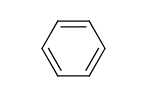
\includegraphics{smile-32fa173088c9c6fbb4d87dcf63069a62635c0f4b}

Các phản ứng trên có thuận lợi về phương diện nhiệt hay không? Phản ứng theo chiều ngược lại có biến thiên enthalpy bằng bao nhiêu?\\
15.9. Bằng cách tính biến thiên enthalpy chuẩn của quá trình sau dựa vào năng lượng liên kết, hãy chỉ ra ở điều kiện chuẩn, $\mathrm{H}_{3} \mathrm{C}-\mathrm{CH}_{2}-\mathrm{OH}$ hay $\mathrm{H}_{3} \mathrm{C}-\mathrm{O}-\mathrm{CH}_{3}$ bền hơn.

$$
\mathrm{H}_{3} \mathrm{C}-\mathrm{CH}_{2}-\mathrm{OH}(g) \rightarrow \mathrm{H}_{3} \mathrm{C}-\mathrm{O}-\mathrm{CH}_{3}(g)
$$

15.10. Xét các phản ứng thế trong dãy halogen ở điều kiện chuẩn:\\
(1) $\frac{1}{2} \mathrm{~F}_{2}(g)+\mathrm{NaCl}(s) \rightarrow \mathrm{NaF}(s)+\frac{1}{2} \mathrm{Cl}_{2}(g)$\\
(2) $\frac{1}{2} \mathrm{Cl}_{2}(g)+\mathrm{NaBr}(s) \rightarrow \mathrm{NaCl}(s)+\frac{1}{2} \mathrm{Br}_{2}(l)$\\
(3) $\frac{1}{2} \mathrm{Br}_{2}(l)+\mathrm{NaI}(s) \rightarrow \mathrm{NaBr}(s)+\frac{1}{2} \mathrm{I}_{2}(s)$\\
(4) $\frac{1}{2} \mathrm{Cl}_{2}(g)+\mathrm{NaBr}(a q) \rightarrow \mathrm{NaCl}(a q)+\frac{1}{2} \mathrm{Br}_{2}(l)$

Hay còn viết: $\frac{1}{2} \mathrm{Cl}_{2}(g)+\mathrm{Br}^{-}(a q) \rightarrow \mathrm{Cl}^{-}(a q)+\frac{1}{2} \mathrm{Br}_{2}(l)$\\
(5) $\frac{1}{2} \mathrm{Br}_{2}(l)+\mathrm{NaI}(a q) \rightarrow \mathrm{NaBr}(a q)+\frac{1}{2} \mathrm{I}_{2}(s)$

Hay còn viết: $\frac{1}{2} \mathrm{Br}_{2}(l)+\mathrm{I}^{-}(a q) \rightarrow \mathrm{Br}^{-}(a q)+\frac{1}{2} \mathrm{I}_{2}(s)$\\
a) Từ các giá trị của enthalpy hình thành chuẩn, hãy tính biến thiên enthalpy chuẩn của các phản ứng thế trên.

\begin{center}
\begin{tabular}{|l|c|c|c|c|c|}
\hline
$\mathrm{Châtl} / \mathrm{lon}$ & $\mathrm{NaF}(s)$ & $\mathrm{NaI}(s)$ & $\mathrm{Cl}(a q)$ & $\mathrm{Br}(a q)$ & $\mathrm{I}(a q)$ \\
\hline
$\Delta_{\mathrm{r}} \mathbf{H}_{2 \mathrm{q}}^{0}\left(\mathbf{k J ~ m o l}^{-1}\right)$ & $-574,0$ & $-287,8$ & $-167,2$ & $-121,6$ & $-55,2$ \\
\hline
\end{tabular}
\end{center}

(Các giá trị khác được cho trong Phụ lục 3, SGK Hoá học 10, Cánh Diều.)\\
b) Nhận xét sự thuận lợi về phương diện nhiệt của các phản ứng thế trong dãy halogen. Kết quả này có phù hợp với quy luật biến đổi tính phi kim của dãy halogen trong bảng tuần hoàn các nguyên tố hoá học không?\\
15.11. Phân tử hemoglobin ( Hb ) trong máu nhận $\mathrm{O}_{2}$ ở phổi để chuyển thành $\mathrm{HbO}_{2}$. Chất này theo máu tới các bộ phận cơ thể, tại đó $\mathrm{HbO}_{2}$ lại chuyển thành Hb và $\mathrm{O}_{2}$ (để cung cấp $\mathrm{O}_{2}$ cho các hoạt động sinh hoá cấn thiết trong cơ thể). Nếu trong không khí có lẫn carbon monoxide ( CO ), cơ thể nhanh chóng bị ngộ độc. Cho các số liệu thực nghiệm sau:

$$
\begin{array}{ll}
\mathrm{Hb}+\mathrm{O}_{2} \rightarrow \mathrm{HbO}_{2} & \Delta_{\mathrm{r}} \mathrm{H}_{298}^{0}=-33,05 \mathrm{~kJ} \\
\mathrm{Hb}+\mathrm{CO} \rightarrow \mathrm{HbCO} & \Delta_{\mathrm{r}} \mathrm{H}_{298}^{0}=-47,28 \mathrm{~kJ} \\
\mathrm{HbO}_{2}+\mathrm{CO} \rightarrow \mathrm{HbCO}+\mathrm{O}_{2} & \Delta_{\mathrm{r}} \mathrm{H}_{298}^{0}=-14,23 \mathrm{~kJ} \\
\mathrm{HbCO}+\mathrm{O}_{2} \rightarrow \mathrm{HbO}_{2}+\mathrm{CO} & \Delta_{\mathrm{r}} \mathrm{H}_{298}^{0}=14,23 \mathrm{~kJ}
\end{array}
$$

Liên hệ giữa mức độ thuận lợi của phản ứng (qua $\Delta_{\mathrm{r}} \mathrm{H}_{298}^{0}$ ) với những vấn đề thực nghiệm nêu trên.

\section*{CHỦ DỀ 6: TỐC ĐỘ PHẢN ỨNG HOÁ HOC}
BMI\\
16 TỐC ĐỘ PHẢN ÚNG HOÁ HOC\\
16.1. Những phát biểu nào sau đây là đúng?\\
A. Tốc độ của phản ứng hoá học là đại lượng mô tả mức độ nhanh hay chậm của chất phản ứng được sử dụng hoặc sản phẩm được tạo thành.\\
B. Tốc độ của phản ứng hoá học là hiệu số nồng độ của một chất trong hỗn hợp phản ứng tại hai thời điểm khác nhau.\\
C. Tốc độ của phản ứng hoá học có thể có giá trị âm hoặc dương.\\
D. Trong cùng một phản ứng hoá học, tốc độ tạo thành của các chất sản phẩm khác nhau là khác nhau, tuỳ thuộc vào hệ số cân bằng của chúng trong phương trình hoá học.\\
E. Trong cùng một phản ứng hoá học, tốc độ tiêu thụ các chất phản ứng khác nhau sẽ như nhau nếu chúng được lấy với cùng một nồng độ.\\
16.2. Những phát biểu nào sau đây không đúng?\\
A. Tốc độ của phản ứng hoá học chỉ có thể được xác định theo sự thay đổi nồng độ chất phản ứng theo thời gian.\\
B. Tốc độ của phản ứng hoá học không thể xác định được từ sự thay đổi nồng độ chất sản phẩm tạo thành theo thời gian.\\
C. Theo công thức tính, tốc độ trung bình của phản ứng hoá học trong một khoảng thời gian nhất định là không thay đổi trong khoảng thời gian ấy.\\
D. Dấu "-" trong biểu thức tính tốc độ trung bình theo biến thiên nồng độ chất phản ứng là để đảm bảo cho giá trị của tốc độ phản ứng không âm.\\
E. Tốc độ trung bình của một phản ứng trong một khoảng thời gian nhất định được biểu thị bằng biến thiên nồng độ chất phản ứng hoặc sản phẩm tạo thành chia cho khoảng thời gian đó.\\
16.3. Khi cho một lượng xác định chất phản ứng vào bình để cho phản ứng hoá học xảy ra, tốc độ phản ứng sẽ\\
A. không đổi cho đến khi kết thúc.\\
B. tăng dần cho đến khi kết thúc.\\
C. chậm dần cho đển khi kết thúc.\\
D. tuân theo định luật tác dụng khối lượng.\\
16.4. Tốc độ phản ứng còn được tính theo sự thay đổi lượng chất (số mol, khối lượng) theo thời gian. Cho hai phản ứng xảy ra đồng thời trong hai bình (1) và (2):


\begin{align*}
& \mathrm{Ca}+\mathrm{Cl}_{2} \rightarrow \mathrm{CaCl}_{2}  \tag{1}\\
& 2 \mathrm{~K}+\mathrm{Cl}_{2} \rightarrow 2 \mathrm{KCl} \tag{2}
\end{align*}


Sau 2 phút, có 3 gam $\mathrm{CaCl}_{2}$ được hình thành theo phản ứng (1).\\
a) Xác định tốc độ trung bình của phản ứng (theo đơn vị mol phút ${ }^{-1}$ ) theo lượng sản phẩm được tạo ra.\\
b) Giả sử phản ứng (2) cũng xảy ra cùng một tốc độ trung bình như phản ứng (1), hãy tính số mol KCl được tạo thành sau 2 phút. Cho biết khối lượng (gam) của K cần thiết để tạo ra số mol KCl trên.\\
16.5. Cho hai phản ứng có phương trình hoá học như sau:


\begin{align*}
2 \mathrm{O}_{3}(g) & \rightarrow 3 \mathrm{O}_{2}(g)  \tag{1}\\
2 \mathrm{HOF}(g) & \rightarrow 2 \mathrm{HF}(g)+\mathrm{O}_{2}(g) \tag{2}
\end{align*}


a) Viết biểu thức tốc độ trung bình (theo cả các chất phản ứng và chất sản phẩm) của hai phản ứng trên.\\
b) Trong phản ứng (1), nếu $\frac{\Delta \mathrm{C}_{\mathrm{O}_{2}}}{\Delta \mathrm{t}}=1,5 \times 10^{-4} \mathrm{~mol} \mathrm{~L}^{-1} \mathrm{~s}^{-1}$ thi $\frac{\Delta \mathrm{C}_{\mathrm{O}_{3}}}{\Delta \mathrm{t}}$ bằng bao nhiêu?\\
16.6. Phản ứng $3 \mathrm{H}_{2}+\mathrm{N}_{2} \rightarrow 2 \mathrm{NH}_{3}$ có tốc độ mất đi của $\mathrm{H}_{2}$ so với tốc độ hình thành $\mathrm{NH}_{3}$ như thế nào?\\
A. Bằng $\frac{1}{2}$.\\
B. Bằng $\frac{3}{2}$.\\
C. Bằng $\frac{2}{3}$.\\
D. Bằng $\frac{1}{3}$.\\
16.7. Cho phản ứng: $\quad 6 \mathrm{CH}_{2} \mathrm{O}+4 \mathrm{NH}_{3} \rightarrow\left(\mathrm{CH}_{2}\right)_{6} \mathrm{~N}_{4}+6 \mathrm{H}_{2} \mathrm{O}$.

Tốc độ trung bình của phản ứng trên được biểu diễn bằng những biểu thức nào trong những biểu thức sau?\\
A. $\frac{1}{6} \frac{\Delta \mathrm{C}_{\mathrm{H}_{2} \mathrm{O}}}{\Delta \mathrm{t}}$.\\
B. $-\frac{1}{4} \frac{\Delta \mathrm{C}_{\mathrm{NH}_{3}}}{\Delta \mathrm{t}}$.\\
C. $\frac{1}{6} \frac{\Delta \mathrm{C}_{\mathrm{CH}_{2} \mathrm{O}}}{\Delta \mathrm{t}}$.\\
D. $-\frac{1}{6} \frac{\Delta \mathrm{C}_{\mathrm{CH}_{2} \mathrm{O}}}{\Delta \mathrm{t}}$\\
E. $-\frac{\Delta \mathrm{C}_{\left(\mathrm{CH}_{2}\right)_{6} \mathrm{~N}_{4}}}{\Delta \mathrm{t}}$.\\
16.8. Những phát biểu nào sau đây không đủng?\\
A. Phản ứng đơn giản là phản ứng xảy ra theo một bước.\\
B. Phản ứng đơn giản là phản ứng có các hệ số tỉ lượng trong phương trình hoá học bằng nhau và bằng 1 .\\
C. Tốc độ của một phản ứng đơn giản tuân theo định luật tác dụng khối lượng.\\
D. Tốc độ của mọi phản ứng hoá học đều tuân theo định luật tác dụng khối lượng.\\
E. Hằng số tốc độ phản ứng là tốc độ của phản ứng khi nồng độ của tất cả các chất trong hỗn hợp phản ứng đều bằng nhau và bằng 1 .\\
G. Hằng số tốc độ của phản ứng phụ thuộc vào thời gian.\\
H. Hằng số tốc độ phản ứng là tốc độ của phản ứng khi nồng độ các chất phản ứng bằng nhau và bằng 1 M .\\
16.9. Cho phản ứng đơn giản:

$$
\mathrm{H}_{2}+\mathrm{I}_{2} \rightarrow 2 \mathrm{HI}
$$

Người ta thực hiện ba thí nghiệm với nồng độ các chất đầu ( $\mathrm{C}_{\mathrm{H}_{2}}$ và $\mathrm{C}_{\mathrm{I}_{2}}$ ) được lấy khác nhau và xác định được tốc độ tạo thành HI trong 20 giây đầu tiên, kết quả cho trong bảng sau:

\begin{center}
\begin{tabular}{|l|l|l|}
\hline
$\mathrm{C}_{\mathrm{n}}, \mathrm{M}$ & C, (M) & $\frac{\Delta \mathrm{C}_{\mathrm{HI}}}{\Delta \mathrm{t}}\left(\mathrm{M} \mathrm{s}^{-1}\right)$ \\
\hline
0,10 & 0,20 & 5,00 \\
\hline
0,20 & 0,20 & 10,00 \\
\hline
0,10 & 0,15 & 3,75 \\
\hline
\end{tabular}
\end{center}

Biểu thức định luật tác dụng viết cho phản ứng trên là:\\
A. $v=1250 \mathrm{C}_{\mathrm{H}_{2}} \mathrm{C}_{\mathrm{I}_{2}}^{2}$.\\
B. $v=125 \mathrm{C}_{\mathrm{H}_{2}} \mathrm{C}_{\mathrm{I}_{2}}$.\\
C. $v=250 \mathrm{C}_{\mathrm{H}_{2}}^{2}$.\\
D. $v=5,0 \mathrm{C}_{\mathrm{H}_{2}} \mathrm{C}_{\mathrm{I}_{2}}$.\\
16.10. Cho phản ứng:

$$
2 \mathrm{~A}+\mathrm{B} \rightarrow 2 \mathrm{M}+3 \mathrm{~N}
$$

a) Hãy viết biểu thức tốc độ trung bình của phản ứng trên theo sự thay đổi nồng độ chất $\mathrm{A}, \mathrm{B}, \mathrm{M}$ và N .\\
b) Nếu biến thiên nồng độ trung bình của chất $\mathrm{M}\left(\frac{\Delta \mathrm{C}_{\mathrm{M}}}{\Delta \mathrm{t}}\right)$ là $1,0 \mathrm{~mol} \mathrm{~L}^{-1} \mathrm{~s}^{-1}$ thì tốc độ trung bình của phản ứng và biến thiên nồng độ trung bình của $N\left(\frac{\Delta C_{N}}{\Delta t}\right), A\left(-\frac{\Delta C_{A}}{\Delta t}\right)$ và $B\left(-\frac{\Delta C_{B}}{\Delta t}\right)$ lần lượt là:\\
A. $2,0 \mathrm{~mol} \mathrm{~L}^{-1} \mathrm{~s}^{-1} ; 4,0 \mathrm{~mol} \mathrm{~L}^{-1} \mathrm{~s}^{-1} ; 6,0 \mathrm{~mol} \mathrm{~L}^{-1} \mathrm{~s}^{-1}$ và $2,0 \mathrm{~mol} \mathrm{~L}^{-1} \mathrm{~s}^{-1}$.\\
B. $0,5 \mathrm{~mol} \mathrm{~L}^{-1} \mathrm{~s}^{-1} ; 1,5 \mathrm{~mol} \mathrm{~L}^{-1} \mathrm{~s}^{-1} ; 1,0 \mathrm{~mol} \mathrm{~L}^{-1} \mathrm{~s}^{-1}$ và $0,5 \mathrm{~mol} \mathrm{~L}^{-1} \mathrm{~s}^{-1}$.\\
C. $1,0 \mathrm{~mol} \mathrm{~L}^{-1} \mathrm{~s}^{-1} ; 1,0 \mathrm{~mol} \mathrm{~L}^{-1} \mathrm{~s}^{-1} ; 1,0 \mathrm{~mol} \mathrm{~L}^{-1} \mathrm{~s}^{-1}$ và $1,0 \mathrm{~mol} \mathrm{~L}^{-1} \mathrm{~s}^{-1}$.\\
D. $2,0 \mathrm{~mol} \mathrm{~L}^{-1} \mathrm{~s}^{-1} ; 4,0 \mathrm{~mol} \mathrm{~L}^{-1} \mathrm{~s}^{-1} ; 3,0 \mathrm{~mol} \mathrm{~L}^{-1} \mathrm{~s}^{-1}$ và $2,0 \mathrm{~mol} \mathrm{~L}^{-1} \mathrm{~s}^{-1}$.\\
16.11. Phản ứng $\mathrm{A} \rightarrow 2 \mathrm{~B}$ được thực hiện trong một bình phản ứng. Số liệu thực nghiệm của phản ứng được cho trong bảng sau:

\begin{center}
\begin{tabular}{|c|c|c|c|c|c|}
\hline
\begin{tabular}{c}
Thờ gian (giây) \\
\hline
\begin{tabular}{c}
Nồng dô chát B \\
(nol L-) \\
\end{tabular} \\
\hline
\end{tabular} & 0,0 & 10,0 & 20,0 & 30,0 & 40,0 \\
\hline
\end{tabular}
\end{center}

a) Hãy tính sự thay đổi nồng độ chất B sau mỗi 10 giây từ 0,0 tới 40,0 giây. Các giá trị này tăng hay giảm khi đi từ khoảng thời gian này sang khoảng thời gian tiếp theo? Vì sao?\\
b) Tốc độ thay đổi của nồng độ chất A có liên quan như thế nào với tốc độ thay đồi nồng độ chất của chất B trong mỗi khoảng thời gian? Tính tốc độ thay đổi nồng độ của A trong khoảng thời gian từ 10,0 đến 20,0 giây.\\
16.12. Bạn $A$ và $B$ thực hiện phản ứng giữa kẽm với dung dịch hydrochloric acid và thu thể tích khí thoát ra theo thời gian. Hai bạn lặp lại thí nghiệm ba lần và kết quả của ba lần thí nghiệm được hai bạn ghi vào bảng sau:

\begin{center}
\begin{tabular}{|l|l|l|l|l|l|}
\hline
\multirow{2}{*}{Thơl gian (s)} & \multicolumn{4}{|c|}{Thé tích khí thu duroc (mL)} & \multirow[b]{2}{*}{$\frac{\Delta V_{k n t}}{\Delta t}$ ( $\Delta t-10 s$ )} \\
\hline
 & Lân 1 & Lần 2 & Lân 3 & Trung binh &  \\
\hline
0 & 0 & 0 & 0 &  &  \\
\hline
10 & 23 & 24 & 25 &  &  \\
\hline
20 & 45 & 43 & 44 &  &  \\
\hline
\end{tabular}
\end{center}

\begin{center}
\begin{tabular}{|l|l|l|l|l|l|}
\hline
\multirow{2}{*}{Thor gian (s)} & \multicolumn{4}{|c|}{Thể tich khí thu đươc (mL)} & \multirow{2}{*}{$\frac{\Delta V_{k b i}}{\Delta t}$ ( $\Delta \mathrm{t}=10 \mathrm{~s}$ )} \\
\hline
 & Lần 1 & Lần 2 & Lần 3 & Trung binh &  \\
\hline
30 & 54 & 56 & 55 &  &  \\
\hline
40 & 65 & 61 & 63 &  &  \\
\hline
50 & 73 & 69 & 70 &  &  \\
\hline
60 & 77 & 75 & 76 &  &  \\
\hline
70 & 77 & 76 & 77 &  &  \\
\hline
\end{tabular}
\end{center}

a) Cho biết khí thoát ra là khí gì. Hãy viết và cân bằng phương trình hoá học của phản ứng xảy ra.\\
b) Hoàn thành hai cột còn trống trong bảng trên. Hãy biểu diễn kết quả của hai bạn lên đồ thị thể tích khí thu được theo thời gian. Vì sao hai bạn lại lặp lại thí nghiệm ba lần?\\
c) Dựa vào đồ thị, cho biết khi nào phản ứng kết thúc. Vì sao?\\
d) Phản ứng diễn ra nhanh nhất trong khoảng thời gian nào? Sau đó, phản ứng diễn ra nhanh dần hay chậm dần?\\
e) Nếu thí nghiệm được lặp lại với nồng độ HCl lớn hơn thì tốc độ phản ứng sẽ nhanh hơn hay chậm hơn?\\
g) Nếu hai bạn không đo được thể tích khí thoát ra, em hãy đề xuất một cách khác để xác định tốc độ phản ứng.\\
16.13. Một phản ứng có hệ số nhiệt độ Van't Hoff bằng $3,5.0^{\circ} 15^{\circ} \mathrm{C}$, tốc độ của phản ứng này bằng $0,2 \mathrm{M} \mathrm{s}^{-1}$. Tính tốc độ của phản ứng ở $40^{\circ} \mathrm{C}$.\\
16.14. Một bạn học sinh thực hiện hai thí nghiệm:

Thí nghiệm 1: Cho 100 mL dung dịch acid HCl vào cốc (1), sau đó thêm một mẫu kẽm và đo tốc độ khí $\mathrm{H}_{2}$ thoát ra theo thời gian.\\
Thí nghiệm 2 (lặp lại tương tự thí nghiệm 1): 100 mL dung dịch acid HCl khác được cho vào cốc (2) rồi cũng thêm một mẫu kẽm vào và lại đo tốc độ khí hydrogen thoát ra theo thời gian.\\
Bạn học sinh đó nhận thấy tốc độ thoát khí hydrogen ở cốc (2) nhanh hơn ở cốc (1).

Những yếu tố nào sau đây có thể dùng để giải thích hiện tượng mà bạn đó quan sát được?\\
A. Phản ứng ở cốc (2) nhanh nhờ có chất xúc tác.\\
B. Lượng kẽm ở cốc (1) nhiều hơn ở cốc (2).\\
C. Acid HCl ở cốc (1) có nồng độ thấp hơn acid ở cốc (2).\\
D. Kẽm ở cốc (2) được nghiền nhỏ còn kẽm ở cốc (1) ở dạng viên.\\
16.15. Khi tăng áp suất của chất phản ứng, tốc độ của những phản ứng nào sau đây sẽ bị thay đổi?\\
A. $2 \mathrm{Al}(s)+\mathrm{Fe}_{2} \mathrm{O}_{3}(s) \rightarrow \mathrm{Al}_{2} \mathrm{O}_{3}(s)+2 \mathrm{Fe}(s)$.\\
B. $2 \mathrm{H}_{2}(g)+\mathrm{O}_{2}(g) \rightarrow 2 \mathrm{H}_{2} \mathrm{O}(l)$.\\
C. $\mathrm{C}(s)+\mathrm{O}_{2}(g) \rightarrow \mathrm{CO}_{2}(g)$.\\
D. $\mathrm{CaCO}_{3}(s)+2 \mathrm{HCl}(a q) \rightarrow \mathrm{CaCl}_{2}(a q)+\mathrm{H}_{2} \mathrm{O}(l)+\mathrm{CO}_{2}(g)$.\\
16.16. Khi nghiên cứu ảnh hưởng của nhiệt độ tới tốc độ của phản ứng giữa $\mathrm{Mg}(s)$ với $\operatorname{HCl}(a q)$, những mô tả nào sau đây phản ánh đúng hiện tượng quan sát được khi làm thí nghiệm?\\
A. Khi đun nóng, bọt khí thoát ra nhanh hơn so với không đun nóng.\\
B. Khi đun nóng, bọt khí thoát ra chậm hơn so với không đun nóng.\\
C. Khi đun nóng, dây Mg tan nhanh hơn so với không đun nóng.\\
D. Khi đun nóng, dây Mg tan chậm hơn so với không đun nóng.\\
16.17. Từ một miếng đá vôi và một lọ dung dịch HCl 1 M , thí nghiệm được tiến hành trong điều kiện nào sau đây sẽ thu được lượng $\mathrm{CO}_{2}$ lớn nhất trong một khoảng thời gian xác định?\\
A. Tán nhỏ miếng đá vôi, cho vào dung dịch HCl 1 M , không đun nóng.\\
B. Tán nhỏ miếng đá vôi, cho vào dung dịch HCl 1 M , đun nóng.\\
C. Cho miếng đá vôi vào dung dịch HCl 1 M , không đún nóng.\\
D. Cho miếng đá vôi vào dung dịch HCl 1 M , đun nóng.\\
16.18. Chất xúc tác là chất\\
A. làm tăng tốc độ phản ứng và không bị mất đi sau phản ứng.\\
B. làm tăng tốc độ phản ứng và bị mất đi sau phản ứng.\\
C. làm giảm tốc độ phản ứng và không bị mất đi sau phản ứng.\\
D. làm giảm tốc độ phản ứng và bị mất đi sau phản ứng.\\
16.19. Enzyme catalase phân huỷ hydrogen peroxide thành oxygen và nước nhanh gấp khoảng $10^{7}$ lần sự phân huỷ khi không có xúc tác. Giả sử một phản ứng không có xúc tác phân huỷ một lượng hydrogen peroxide mất 360 ngày, hãy tính thời gian (theo giây) cho sự phân huỷ cùng một lượng hydrogen peroxide đó khi sử dụng enzyme catalase làm xúc tác.\\
16.20. Hai bạn Tôm và Vừng thực hiện một thí nghiệm về sự phân huỷ của hydrogen peroxide với chất xúc tác manganese dioxide ( $\mathrm{MnO}_{2}$ ), Hai bạn thấy rằng phản ứng sủi bọt nhiều và khí thoát ra mạnh khi thêm manganese dioxide.

\begin{enumerate}
  \item Hoàn thành các câu sau đây nói về thí nghiệm của hai bạn.\\
a) Phương trình của phản ứng là: ......\\
b) Chất khí thoát ra là ...(1)... và có thể kiểm tra (nhận biết) ra nó bằng cách ...(2)...\\
c) Sau một thời gian nhất định, Vừng nói với Tôm là phản ứng đã kết thúc vì ......\\
d) Hai bạn biết rằng chất xúc tác chỉ làm tăng tốc độ phản ứng mà không thay đổi về bản chất hoá học nên Tôm sẽ thu lại manganese dioxide sau khi phản ứng kết thúc bằng cách ......
  \item Tôm và Vừng muốn biết liệu cho lượng xúc tác nhiều hơn thì có làm phản ứng nhanh hơn không. Em hãy đề xuất một kế hoạch thí nghiệm cho nghiên cứu của hai bạn. Trong bản kế hoạch, em cần viết cả những lưu ý để đảm bảo an toàn khi làm việc trong phòng thí nghiệm.
\end{enumerate}

\section*{CHỦ DỀ 7: NGUYÊN TỐ NHÓM VIIA (NHÓM HALOGEN)}
\section*{BAT 17}
NGUYÊN TỐ VÀ DƠN CHẤT HALOGEN\\
17.1. Phát biểu nào sau đây không đúng khi nói về nguyên tử các nguyên tố nhóm VIIA?\\
A. Có 7 electron hoá trị.\\
B. Theo chiều tăng dần điện tích hạt nhân nguyên tử thì độ âm điện giảm.\\
C. Theo chiều tăng dần điện tích hạt nhân nguyên tử thì khả năng hút cặp electron liên kết giảm.\\
D. Theo chiều tăng dần điện tích hạt nhân nguyên tử thì bán kính nguyên tử giảm.\\
17.2. a) Điền tên và kí hiệu nguyên tố các halogen bền vào vị trí các nguyên tố A , $\mathrm{B}, \mathrm{C}, \mathrm{D}$ bên đưới. Biết mỗi vòng tròn minh hoạ cho một nguyên tử với tỉ lệ kích thước tương ứng.

\begin{figure}[h]
\begin{center}
  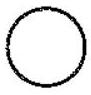
\includegraphics[width=\textwidth]{2025_10_23_76620c17ffac1ae9b35bg-54(1)}
\captionsetup{labelformat=empty}
\caption{A $\_\_\_\_$}
\end{center}
\end{figure}

\begin{figure}[h]
\begin{center}
  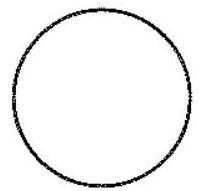
\includegraphics[width=\textwidth]{2025_10_23_76620c17ffac1ae9b35bg-54(3)}
\captionsetup{labelformat=empty}
\caption{B $\_\_\_\_$}
\end{center}
\end{figure}

\begin{figure}[h]
\begin{center}
  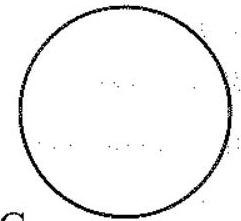
\includegraphics[width=\textwidth]{2025_10_23_76620c17ffac1ae9b35bg-54(2)}
\captionsetup{labelformat=empty}
\caption{C $\_\_\_\_$}
\end{center}
\end{figure}

\begin{figure}[h]
\begin{center}
  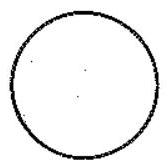
\includegraphics[width=\textwidth]{2025_10_23_76620c17ffac1ae9b35bg-54}
\captionsetup{labelformat=empty}
\caption{D $\_\_\_\_$}
\end{center}
\end{figure}

b) Viết công thức phân tử đơn chất của mỗi nguyên tố tương ứng.\\
c) Ở điều kiện nhiệt độ, áp suất thông thường, các đơn chất này tồn tại ở trạng thái nào? Từ đó, dự đoán thứ tự tăng nhiệt độ nóng chảy, nhiệt độ sôi tương ứng giữa chúng trong cùng điều kiện áp suất.\\
17.3. Nguyên nhân dẫn tới nhiệt độ nóng chảy, nhiệt độ sôi của các đơn chất halogen tăng từ fluorine đến iodine là do từ fluorine đến iodine,\\
A. khối lượng phân tử và tương tác van der Waals đều tăng.\\
B. tính phi kim giảm và tương tác van der Waals tăng.\\
C. khối lượng phân tử tăng và tương tác van der Waals giảm.\\
D. độ âm điện và tương tác van der Waals đều giảm.\\
17.4. Phát biểu nào sau đây là không đúng khi nói về đơn chất nhóm VIIA?\\
A. Tính chất đặc trưng là tính oxi hoá.\\
B. Màu sắc đậm dần từ fluorine đến iodine.\\
C. Từ fluorine đến bromine rồi iodine, trạng thái của các đơn chất chuyển từ khí đến lỏng rồi rắn.\\
D. Khả năng phản ứng với nước tăng từ fluorine đến iodine.\\
17.5. Những phát biểu nào sau đây là đúng khi nói về tính chất và phản ứng của đơn chất nhóm VIIA?\\
A. Tính oxi hoá giảm dần từ fluorine đến iodine.\\
B. Phản ứng với nhiều kim loại, tạo thành hợp chất ion. Phản ứng với một số phi kim, tạo thành hợp chất cộng hoá trị.\\
C. Khi phản ứng với đơn chất hydrogen, các đơn chất nhóm VIIA thể hiện tính khử.\\
D. Khi phản ứng với đơn chất hydrogen, mức độ phản ứng giảm dần từ fluorine đến iodine.\\
17.6. Nối mỗi chất trong cột A với những tính chất tương ứng của chúng trong cột B.

\section*{Cột A}
a) Chlorine, $\mathrm{Cl}_{2}$\\
b) Iodine, $I_{2}$

\section*{Cột B}
\begin{enumerate}
  \item Hầu như không tan trong nước.
  \item Là chất khí ở điều kiện thường.
  \item Là chất rắn ở điều kiện thường.
  \item Là chất oxi hoá khi phản ứng với kim loại.
  \item Có độc tính cao.
  \item Có tương tác van der Waals mạnh nhất trong nhóm đơn chất halogen.
  \item Dùng để xử lí nước sinh hoạt.\\
17.7. Những phát biểu nào sau đây là đúng khi nói về phản ứng của đơn chất halogen với hydrogen?\\
A. Các phản ứng đều phát nhiệt mạnh và kèm hiện tượng nổ.\\
B. Phản ứng giữa fluorine với hydrogen diễn ra mãnh liệt nhất.\\
C. Điều kiện và mức độ phản ứng phù hợp với xu hướng giảm dần tính oxi hoá từ fluorine đến iodine.\\
D. Do hợp chất hydrogen iodide sinh ra kém bền (giá trị năng lượng liên kết nhỏ) nên phản ửng giữa iodine với hydrogen là phản ứng hai chiều.\\
17.8. Những phát biểu nào sau đây là đúng khi nói về phản ứng của đơn chất nhóm VIIA với nước?\\
A. Các đơn chất nhóm VIIA vưa thể hiện tính oxi hoá, vừa thể hiện tính khử; mức độ phản ứng giảm dần từ fluorine đến iodine.\\
B. Fluorine phản ứng rất mạnh với nước tạo dung dịch có tính oxi hoá mạnh, có thể dùng để sát khuẩn.\\
C. Phản úng của bromine hoặc chlorine với nước đều là phản ứng thuận nghịch.\\
D. Iodine tan rất ít và hầu như không phản ứng với nước.\\
17.9. Phát biểu nào sau đây là không đúng khi nói về phản ứng của đơn chất nhóm VIIA với dung dịch muối halide?\\
A. Bromine phản ứng dễ dàng với dung dịch sodium fluoride để tạo ra đơn chất fluorine.\\
B. Khi cho vào dung dịch sodium chloride, fluorine sẽ ưu tiên phản ứng với nước.\\
C. Có thể sục khí chlorine vào dung dịch chứa potassium iodide để thu được iodine.\\
D. Iodine khó tan trong dung dịch sodium chloride.\\
17.10. Phát biểu nào sau đây là không đúng khi nói về một số ứng dụng của đơn chất chlorine?\\
A. Khí chlorine có thể được dùng để tạo môi trường sát khuẩn cho nguồn nước cấp.\\
B. Khí chlorine phản ứng với đung dịch sodium hydroxide tạo dung dịch nước Javel dùng để sát khuẩn trong công nghiệp và trong gia đình.\\
C. Khí chlorine được sử dụng để sản xuất hydrogen chloride, từ đó tạo hydrochloric acid.\\
D. Do có độc tính, khí chlorine được sử dụng để trừ sâu trong nông nghiệp.\\
17.11. Những phát biếu nào sau đây là đúng?\\
A. Đơn chất chlorine có tính oxi hoá mạnh hơn đơn chất bromine và iodine.\\
B. Tương tác van der Waals của các đơn chất halogen tăng từ fluorine đến iodine đã góp phần làm tăng nhiệt độ sôi của chúng.\\
C. Thành phần của nước bromine gồm các chất: $\mathrm{Br}_{2}, \mathrm{H}_{2} \mathrm{O}, \mathrm{HBr}, \mathrm{HBrO}$.\\
D. Hoá trị phổ biến của nguyên tố halogen là I.\\
E. Đơn chất iodine phản ứng được với nước và với dung dịch sodium bromide.\\
17.12. Nhúng giấy quỳ vào dung dịch nước chlorine thì thấy giấy quỳ chuyển sang màu đỏ. Nhưng ngay sau đó, màu đỏ trên giấy quỳ sẽ biến mất. Hãy giải thích hiện tượng này.\\
17.13. Ở các đô thị, khi thay nước cho các bồn nuôi cá cảnh, người ta không cho trực tiếp nước sinh hoạt (nước máy) vào bồn cá. Nước này phải được chứa trong xô, thau, chậu khoảng một ngày rồi mới được cho vào bồn nuôi cá. Hãy giải thích.\\
17.14*. Để bảo đảm vệ sinh, nước ở các hồ bơi thường xuyên được xử lí bằng hoá chất. Hãy tìm hiểu và cho biết:\\
a) Các hoá chất nào thường được sử dụng để xử lí vi khuẩn có trong nước hồ bơi?\\
b) Nhờ đâu mà các hoá chất ấy giúp xử li vi khuẩn có trong nước hồ bơi?\\
c) Để bảo đảm an toàn cho người bơi trong hồ, cần lưu ý gì khi sử dụng các hoá chất ấy?\\
17.15. Thổi một lượng khí chlorine vào dung dịch chứa m gam hai muối bromide của sodium và potassium. Sau khi phản ứng xảy ra hoàn toàn, cô cạn dung dịch, khối lượng chất rắn thu được giảm 4,45 gam so với lượng muối trong dung dịch ban đầu. Chọn phát biểu đúng về số mol khí chlorine đã tham gia phản ứng với các muối trên.\\
A. $0,10 \mathrm{~mol}$.\\
B. Ít hơn $0,06 \mathrm{~mol}$.\\
C. Nhiều hơn $0,12 \mathrm{~mol}$.\\
D. $0,07 \mathrm{~mol}$.\\
17.16. a) Trong công nghiệp, xút (sodium hydroxide) được sản xuất bằng phương pháp điện phân dung dịch sodium chloride có màng ngăn xốp. Bằng phương pháp này, người ta cũng thu được khí chlorine (sơ đồ minh hoạ). Chất khí này được làm khô (loại hơi nước) rồi hoá lỏng để làm nguyên liệu quan trọng cho nhiều ngành công nghiệp chế biến và sản xuất hoá chất. Theo em, chất nào sau đây phù hợp để làm khô khí chlorine?\\
A. Sulfuric acid $98 \%$.\\
B. Sodium hydroxide khan.\\
C. Calcium oxide khan.\\
D. Dung dịch sodium chloride bão hoà.\\
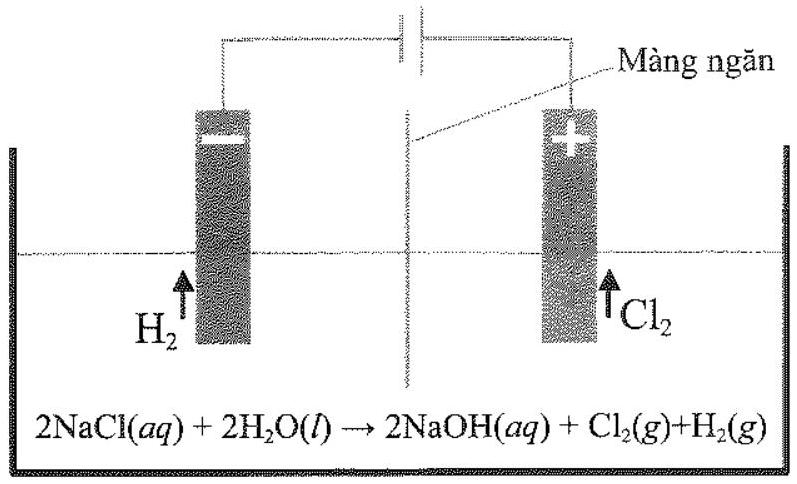
\includegraphics[max width=\textwidth, center]{2025_10_23_76620c17ffac1ae9b35bg-58}\\
b) Từ quá trình điện phân nêu trên, một lượng chlorine và hydrogen sinh ra được tận dụng để sản xuất hydrochloric acid đặc thương phẩm ( $32 \%$, $\mathrm{D}=1,153 \mathrm{~g} \mathrm{~mL}^{-1}$ ở $30^{\circ} \mathrm{C}$ ).\\
Một nhà máy với quy mô sản xuất 200 tấn xút mỗi ngày thì đồng thời sản xuất được bao nhiêu $\mathrm{m}^{3}$ acid thương phẩm trên. Biết rằng, tại nhà máy này, $60 \%$ khối lượng chlorine sinh ra được dùng tổng hợp hydrochloric acid và hiệu suất của toàn bộ quá trình từ chlorine đến acid thương phẩm đạt $80 \%$ về khối lượng.\\
17.17. Iodine là chất rắn, ít tan trong nước, nhưng lại tan khá dễ dàng trong dung dịch potassium iodide là do phản ứng sau:
\end{enumerate}

$$
\mathrm{I}_{2}(s)+\mathrm{KI}(a q) \rightarrow \mathrm{KI}_{3}(a q)
$$

Vai trò của KI trong phản ứng trên là gì?\\
A. Chất oxi hoá.\\
B. Chất khử.\\
C. Vừa là chất oxi hoá, vừa là chất khử.\\
D. Không phải chất oxi hoá cũng không phải chất khử.\\
17.18. Calcium chloride hypochlorite $\left(\mathrm{CaOCl}_{2}\right)$ thường được sử dụng làm chất khử trùng bể bơi do có tính oxi hoá mạnh tương tự nước Javel. Tìm hiểu về công thức cấu tạo của $\mathrm{CaOCl}_{2}$, từ đó, biết được số oxi hoá của nguyên tử chlorine trong hợp chất trên là\\
A. +1 và -1 .\\
B. -1 .\\
C. 0 và -1 .\\
D. 0 .\\
17.19. Xét các phản ứng:


\begin{equation*}
\mathrm{X}_{2}(g)+\mathrm{H}_{2}(g) \rightarrow 2 \mathrm{HX}(g) \quad \Delta_{\mathrm{r}} \mathrm{H}_{298}^{0} \tag{}
\end{equation*}


với X lần lượt là $\mathrm{Cl}, \mathrm{Br}, \mathrm{I}$.

Giá trị năng lượng liên kết ( $\mathrm{kJ} \mathrm{mol}^{-1}$ ) một số chất được cho trong Phụ lục 2, SGK Hoá học 10, Cánh Diều.\\
a) Hãy tính biến thiên enthalpy chuẩn của mỗi phản ửng (\textit{).\\
b) Hãy sắp xếp các phản ứng (}) theo thứ tự giảm dần của lượng nhiệt toả ra.\\
17.20. Từ bảng giá trị năng lượng liên kết $\left(\mathrm{kJ} \mathrm{mol}^{-1}\right)$ dưới đây:

\begin{center}
\begin{tabular}{|c|c|c|c|c|}
\hline
$\mathrm{F}-\mathrm{F}$ & $\mathrm{H}-\mathrm{H}$ & $\mathrm{O}_{2}$ & $\mathrm{H}-\mathrm{F}$ & $\mathrm{O}-\mathrm{H}$ \\
\hline
159 & 436 & 498 & 565 & 464 \\
\hline
\end{tabular}
\end{center}

Hãy cho biết:\\
a) Liên kết nào bền nhất, liên kết nào kém bền nhất?\\
b) Giá trị biến thiên enthalpy chuẩn của hai phản ứng sau là bao nhiêu?


\begin{align*}
& \mathrm{F}_{2}(g)+\mathrm{H}_{2}(g) \rightarrow 2 \mathrm{HF}(g)  \tag{1}\\
& \mathrm{O}_{2}(g)+2 \mathrm{H}_{2}(g) \rightarrow 2 \mathrm{H}_{2} \mathrm{O}(g) \tag{2}
\end{align*}


c) Trong hai phản ứng (1) và (2), phản ứng nào toả nhiệt nhiều hơn?\\
17.21. Người ta thường tách bromine trong rong biển bằng quá trình sục khí chlorine vào dung dịch chiết chứa ion bromide. Phương trình hoá học của phản ứng có thể được mô tả dạng thu gọn như sau:

$$
2 \mathrm{Br}^{-}(a q)+\mathrm{Cl}_{2}(a q) \rightarrow 2 \mathrm{Cl}^{-}(a q)+\mathrm{Br}_{2}(a q)
$$

Cho các số liệu enthalpy tạo thành chuẩn $\Delta_{\mathrm{f}} \mathrm{H}_{298}^{0}\left(\mathrm{~kJ} \mathrm{~mol}^{-1}\right)$ trong bảng dưới đây:

\begin{center}
\begin{tabular}{|c|c|c|c|}
\hline
$\mathrm{Br}^{-}(a q)$ & $\mathrm{Cl}^{-}(a q)$ & $\mathrm{Br}_{2}(a q)$ & $\mathrm{Cl}_{2}(a q)$ \\
\hline
$-121,55$ & $-167,16$ & $-2,16$ & $-17,30$ \\
\hline
\end{tabular}
\end{center}

a) Tính biến thiên enthalpy chuẩn phản ứng trên.\\
b) Phản ửng trên có thuận lợi về năng lượng không?\\
17.22. Hình sau đây là một phần phổ khối lượng của chlorine. Phổ này có hai tín hiệu, là hai đường thẳng xuất phát từ toạ độ 35 và 37 trên trục hoành. Nhờ đó, người ta biết được nguyên tố chlorine có hai đồng vị bền là ${ }^{35} \mathrm{Cl}$ và ${ }^{37} \mathrm{Cl}$. Tỉ lệ số nguyên tử của hai đồng vị cũng là tỉ lệ độ cao $\mathrm{h}_{1}$ và $\mathrm{h}_{2}$ (hay tỉ lệ cường độ tương đối) của hai tín hiệu:

$$
\frac{\text { Số nguyên tử }{ }^{35} \mathrm{Cl}}{\text { Số nguyên từ }{ }^{37} \mathrm{Cl}}=\frac{\mathrm{h} 1}{\mathrm{~h} 2}\left({ }^{*}\right)
$$

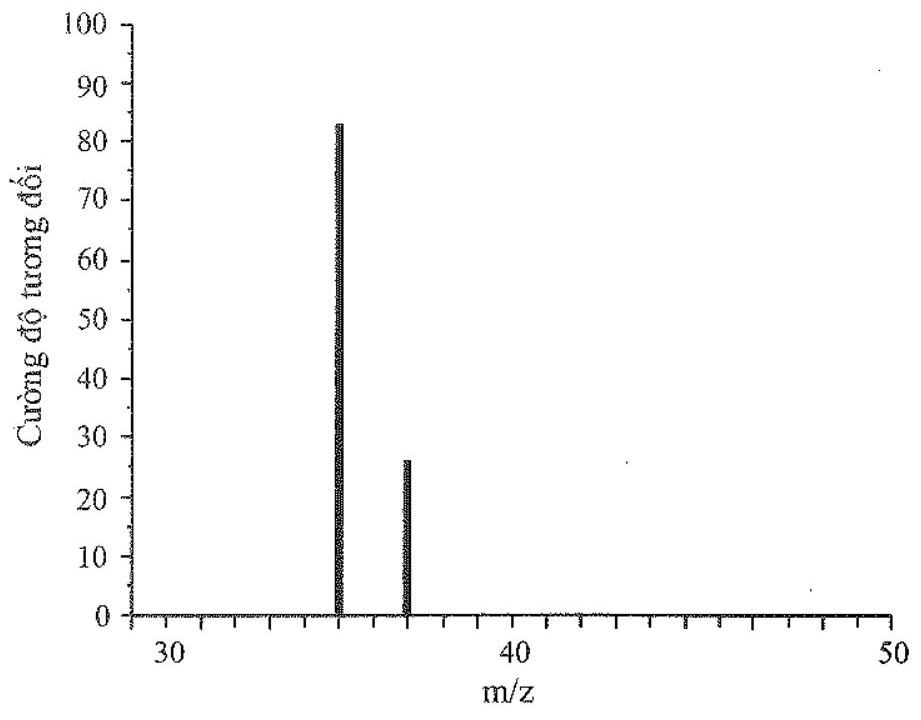
\includegraphics[max width=\textwidth, center]{2025_10_23_76620c17ffac1ae9b35bg-60}\\
a) Dùng thước (độ chia nhỏ nhất là mm ) để đo h 1 và h 2 . Từ đó tính tỉ lệ $\mathrm{h} 1: \mathrm{h} 2$.\\
b) Số nguyên tử đồng vị ${ }^{35} \mathrm{Cl}$ gấp bao nhiêu lần số nguyên tử đồng vị ${ }^{37} \mathrm{Cl}$ ?\\
c) Xác định phần trăm số nguyên tử của mỗi đồng vị.\\
d) Xác định nguyên tử khối trung bình của chlorine.

\section*{Bai 18 HYDROGEN HALIDE VÀ HYDROHALIC ACID}
18.1. Những phát biểu nào dưới đây là đúng khi nói về các hydrogen halide HX ?\\
A. Ở điều kiện thường, đều là chất khí.\\
B. Các phân tử đều phân cực.\\
C. Nhiệt độ sôi tăng từ hydrogen chloride đến hydrogen iodide, phù hợp với xu hướng tăng tương tác van der Waals từ hydrogen chloride đến hydrogen iodide.\\
D. Đều tan tốt trong nước, tạo các dung dịch hydrohalic acid tương ứng.\\
E. Năng lượng liên kết tăng dần từ HF đến HI.\\
18.2. Ở cùng điều kiện áp suất, hydrogen fluoride (HF) có nhiệt độ sôi cao vượt trội so với các hydrogen halide còn lại là do\\
A. fluorine có nguyên tử khối nhỏ nhất.\\
B. năng lượng liên kết H-F bền vững làm cho HF khó bay hơi.\\
C. các nhóm phân tử HF được tạo thành do có liên kết hydrogen giữa các phân tử.\\
D. fluorine là phi kim mạnh nhất.\\
18.3. Những phát biểu nào dưới đây là không đúng khi nói về các hydrohalic acid?\\
A. Đều là các acid mạnh.\\
B. Độ mạnh của acid tăng từ hydrofluoric acid đến hydroiodic acid, phù hợp xu hướng giảm độ bền liên kết từ HF đến HI.\\
C. Hoà tan được các oxide của kím loại, phản ứng được với các hydroxide kim loại.\\
D. Hoà tan được tất cả các kim loại.\\
E. Tạo môi trường có pH lớn hơn 7.\\
18.4. Những phát biểu nào sau đây là đúng khi nói về ion halide $\mathrm{X}^{-}$?\\
A. Dùng dung dịch silver nitrate sẽ phân biệt được các ion $\mathrm{F}^{-}, \mathrm{Cl}^{-}, \mathrm{Br}^{-}, \mathrm{I}^{-}$.\\
B. Với sulfuric acid đặc, các ion $\mathrm{Cl}^{-}, \mathrm{Br}^{-}, \mathrm{I}^{-}$thể hiện tính khử, ion $\mathrm{F}^{-}$không thể hiện tính khử.\\
C. Tính khử của các ion halide tăng theo dãy: $\mathrm{Cl}^{-}, \mathrm{Br}^{-}, \mathrm{I}^{-}$.\\
D. Ion $\mathrm{Cl}^{-}$kết hợp ion $\mathrm{Ag}^{+}$tạo AgCl là chất không tan, màu vàng.\\
18.5. Những phát biểu nào sau đây là không đúng khi nói về ứng dụng hiện nay của một số hydrogen halide và hydrohalic acid?\\
A. Hằng năm, cần hàng chục triệu tấn hydrogen chloride để sản xuất hydrochloric acid.\\
B. Lượng lớn hydrochloric acid sử dụng trong sản xuất nhựa, phân bón, thuốc nhuộm,...\\
C. Hydrochloric acid được sử dụng cho quá trình thuỷ phân các chất trong sản xuất, chế biến thực phẩm.\\
D. Hydrofluoric acid hoặc hydrogen fluoride phản ứng với chlorine dùng để sản xuất fluorine.\\
E. Trong công nghiệp, hydrofluoric acid dùng tẩy rửa các oxide của sắt trên bề mặt của thép.\\
G. Hydrogen fluoride được dùng để sản xuất chất làm lạnh hydrochlorofluorocarbon HCFC (thay thế chất CFC ), chất chảy cryolite,...\\
18.6. Những tính chất nào dưới đây thể hiện tính acid của hydrochloric acid?\\
A. Phản ứng với các hydroxide.\\
B. Hoà tan các oxide của kim loại.\\
C. Hoà tan một số kim loại.\\
D. Phản ứng với phi kim.\\
E. Làm quỳ tím hoá đỏ và tạo môi trường $\mathrm{pH}>7$.\\
G. Phân li ra ion $\mathrm{H}^{+}$.\\
H. Khi phản ứng với kim loại thì tạo ra muối và khí hydrogen.\\
18.7. Nối mỗi chất trong cột A với tính chất tương ứng của chúng trong cột B cho phù hợp.

\section*{Cột A}
a) Hydrogen fluoride\\
b) Hydrofluoric acid\\
c) Hydrogen chloride\\
d) Hydrochloric acid

\section*{Cột B}
\begin{enumerate}
  \item Là chất khí ở điều kiện thường.
  \item Các phân tử tạo liên kết hydrogen với nhau.
  \item Có nhiệt độ sôi cao nhất trong dãy hydrogen halide.
  \item Là acid mạnh.
  \item Ăn mòn thuỷ tinh.
  \item Thường được dùng để thuỷ phân các chất trong quá trình sản xuất.
  \item Hoà tan calcium carbonate có trong đá vôi, magnesium hydroxide, copper(II) oxide.\\
18.8. Những phát biểu nào sau đây là đúng?\\
A. Khi cho potassium bromide rắn phản ứng với sulfuric acid đặc thu được khí hydrogen bromide.\\
B. Hydrofluoric acid không nguy hiểm vì nó là một acid yếu.\\
C. Trong phản ứng điều chế nước Javel bằng chlorine và sodium hydroxide, chlorine vừa đóng vai trò chất oxi hoá, vừa đóng vai trò chất khử.\\
D. Fluorine có số oxi hoá bằng -1 trong các hợp chất.\\
E. Tất cả các muối halide của bạc $(\mathrm{AgF}, \mathrm{AgCl}, \mathrm{AgBr}, \mathrm{AgI})$ đều là những chất không tan trong nước ở nhiệt độ thường.\\
G. Ở cùng điều kiện áp suất, hydrogen fluoride (HF) có nhiệt độ sôi cao nhất trong các hydrogen halide là do liên kết $\mathrm{H}-\mathrm{F}$ bền nhất trong các liên kết $\mathrm{H}-\mathrm{X}$.\\
18.9. Các phân tử HX đều phân cực, nhưng chỉ có các phân tử HF tạo được liên kết hydrogen với nhau. Giải thích.\\
18.10. Hãy đề xuất cách phân biệt bốn dung dịch hydrohalic acid bằng phưong pháp hoá học.\\
18.11. Hoàn thành phương trình hoá học của mỗi phản ứng sau:\\
a) $\mathrm{HCl}(a q)+\mathrm{KMnO}_{4}(s) \rightarrow \mathrm{KCl}(a q)+\mathrm{MnCl}_{2}(a q)+\mathrm{Cl}_{2}(g)+\mathrm{H}_{2} \mathrm{O}(l)$\\
b) $\mathrm{MnO}_{2}(s)+\mathrm{HCl}(a q) \rightarrow \mathrm{MnCl}_{2}(a q)+?+\mathrm{H}_{2} \mathrm{O}(l)$\\
c) $\mathrm{Cl}_{2}(g)+? \rightarrow ?+\mathrm{NaClO}_{3}(a q)+\mathrm{H}_{2} \mathrm{O}(l)$\\
d) $\mathrm{NaBr}(a q)+\mathrm{H}_{2} \mathrm{SO}_{4}(l) \rightarrow \mathrm{NaHSO}_{4}(s)+?+\mathrm{SO}_{2}(g)+\mathrm{H}_{2} \mathrm{O}(g)$\\
e) $\mathrm{HI}(g)+? \rightarrow \mathrm{I}_{2}(g)+\mathrm{H}_{2} \mathrm{~S}(g)+\mathrm{H}_{2} \mathrm{O}(l)$\\
18.12. Điền vào chỗ trống tên gọi hoặc công thức phân tử của các chất tương ứng:\\
a) $\_\_\_\_$ : HI\\
b) $\_\_\_\_$ $: \mathrm{NaCl}$\\
c) Potassium iodide: $\_\_\_\_$ d) $\_\_\_\_$ : NaClO\\
18.13. a) X là các nguyên tố bền thuộc nhóm halogen. Hãy điền công thức hoá học của nguyên tố, chất, ion theo thứ tự với các tính chất tương ứng theo bảng sau:
\end{enumerate}

\begin{center}
\begin{tabular}{|l|l|l|l|l|}
\hline
Timb chát & \multicolumn{4}{|c|}{\begin{tabular}{l}
$\xrightarrow{\text { Chiều tăng tính chất }}$ \\
Chiều tăng tính chất $\longrightarrow$ \\
\end{tabular}} \\
\hline
Độ âm điện nguyên tố X &  &  &  & F \\
\hline
Tính oxi hoá của đơn chất $\mathrm{X}_{2}$ &  &  &  &  \\
\hline
Tính khử của ion $\mathrm{X}^{-}$ &  &  &  &  \\
\hline
Tính acid của hợp chất HX &  &  &  &  \\
\hline
\end{tabular}
\end{center}

b) Viết các phản ứng chứng minh sự thay đổi tính khử của các ion $\mathrm{X}^{-}$theo xu hướng trong bảng đã được hoàn thành ở câu a.\\
c) Tìm hiểu và giải thích vì sao tính acid của các hợp chất HX lại thay đổi theo thứ tự như câu a.\\
18.14. Mỗi năm, hàng triệu tấn hydrochloric acid được cho phản ứng với acetylene (hay ethyne) và ammonia.\\
a) Viết phương trình hoá học của hai phản ứng trên.\\
b) Hai phản ứng trên được dùng trong lĩnh vực sản xuất nào?\\
18.15. Một trong những ứng dụng quan trọng của hydrochloric acid là dùng để loại bỏ gỉ trên thép trước khi đem cán, mạ điện,... Theo đó, thép sẽ được ngâm trong hydrochloric acid nồng độ khoảng $18 \%$ theo khối lượng. Các oxide tạo lớp gỉ trên bề mặt của thép, chủ yếu là các oxide của sắt và một phần sắt sẽ bị hoà tan bởi acid. Quá trình này thu được dung dịch (gọi là dung dịch A ),\\
chủ yếu chứa hydrochloric acid dư và iron(II) chloride được tạo ra từ phản ứng sắt khử ion $\mathrm{Fe}^{3+}$.\\
a) Viết phương trình hoá học của các phản úng diễn ra. Các phản ứng này có phát thải khí độc vào môi trường không?\\
b) Để tái sử dụng acid, dung dịch A được đưa đến thiết bị phun, ở khoảng $180^{\circ} \mathrm{C}$ để thực hiện phản ứng:

$$
4 \mathrm{FeCl}_{2}+4 \mathrm{H}_{2} \mathrm{O}+\mathrm{O}_{2} \rightarrow 8 \mathrm{HCl}+2 \mathrm{Fe}_{2} \mathrm{O}_{3}
$$

Sau quá trình trên, cần làm thế nào để thu được hydrochloric acid?\\
18.16. Xét phản úng sau:

$$
4 \mathrm{HI}(a q)+\mathrm{O}_{2}(g) \rightarrow 2 \mathrm{H}_{2} \mathrm{O}(l)+2 \mathrm{I}_{2}(s)
$$

Cho giá trị enthalpy tạo thành chuẩn ( $\mathrm{kJ} \mathrm{mol}^{-1}$ ) của một số chất trong bảng dưới đây:

\begin{center}
\begin{tabular}{|c|c|c|c|}
\hline
$\mathrm{HI}(a q)$ & $\mathrm{H}_{2} \mathrm{O}(l)$ & $\mathrm{O}_{2}(g)$ & $\mathrm{I}_{2}(s)$ \\
\hline
-55 & -285 & $?$ & $?$ \\
\hline
\end{tabular}
\end{center}

a) Điền giá trị phù hợp vào ô còn trống.\\
b) Xác định biến thiên enthalpy chuẩn của phản ứng trên.\\
c) Nếu chỉ dựa vào giá trị biến thiên enthalpy chuẩn thì phản ứng trên có thuận lợi về mặt năng lượng không? Từ đó, hãy dự đoán hiện tượng xảy ra khi dung dịch hydroiodic acid tiếp xúc không khí.\\
d) Thực tế, người ta phải chứa hydroiodic acid trong chai, lọ được đậy kín. Hãy giải thích.\\
18.17. Trong phòng thí nghiệm, hydrochloric acid đặc có thể được dùng để điều chế khí chlorine theo hai phản ứng sau:


\begin{align*}
& 16 \mathrm{HCl}(a q)+2 \mathrm{KMnO}_{4}(s) \rightarrow 2 \mathrm{MnCl}_{2}(a q)+2 \mathrm{KCl}(a q)+8 \mathrm{H}_{2} \mathrm{O}(l)+5 \mathrm{Cl}_{2}(g) \text { (1) } \\
& 4 \mathrm{HCl}(a q)+\mathrm{MnO}_{2}(s) \rightarrow \mathrm{MnCl}_{2}(a q)+2 \mathrm{H}_{2} \mathrm{O}(l)+\mathrm{Cl}_{2}(g) \tag{2}
\end{align*}


Cho bảng giá trị enthalpy tạo thành chuẩn ( $\mathrm{kJ} \mathrm{mol}^{-1}$ ) của các chất như dưới đây:

\begin{center}
\begin{tabular}{|c|c|c|c|c|c|}
\hline
$\mathrm{HCl}(a q)$ & $\mathrm{KMnO}_{4}(s)$ & $\mathrm{MnO}_{2}(s)$ & $\mathrm{MnCl}_{2}(a q)$ & $\mathrm{KCl}(a q)$ & $\mathrm{H}_{2} \mathrm{O}(l)$ \\
\hline
-167 & -837 & -520 & -555 & -419 & -285 \\
\hline
\end{tabular}
\end{center}

a) Hãy tính biến thiên enthalpy chuẩn của mỗi phản ứng.\\
b) Thực tế, không cần đun nóng, hai phản ứng trên vẫn diễn ra ở nhiệt độ phòng. Vậy phản ứng trên có thể đã thu nhiệt từ đâu?


\end{document}